


%%%%%%%%%%%%%%%%%%%%%%%%%%%
\chapter {Black Virus Disinfection in Triple Loops}
\label{TL}
%%%%%%%%%%%%%%%%%%%%%%%%%%%
 

\section{Introduction}
In this chapter, we discuss parallel strategy on BVD problem in chordal ring. A chordal ring is a circulant graph with $d_1=1$, i.e., it is an augmented ring, and will be denoted by $C_n(1, d_2, ..., d_k)$. More specifically, in chordal ring each node is directly connected to the nodes at distance $d_i$ and $n-d_i$ by additional links called chords. The link connecting two nodes is labeled by the distance that separate these two nodes on the ring. 
For convenience, if we say the agents or the clones move along chord $i$, then they actually move along $d_i$. If we say the agents or the clones move $i$, then they actually move along chord $d_x$ with its length equal to $i$. Let us donated by $d$ the half degree of the chordal ring (for example, for the chordal ring structure $C_n(1,2,4,5)$, $d=4$), by $l$ the length of the longest chord of the chordal ring (for example, for the chordal ring structure $C_n(1,2,4,5)$, $l=5$). In order to simplify the process, we assume that all the nodes in the network are marked with a number: the starting point is marked 0, then the second node is marked 1... Our goal is to minimize the time to complete the whole decontamination process and at the same time the casualties (number of agents destroyed by the BV) In order to do that, we propose parallel strategy for decontaminating the chordal ring.
In the elimination phase, we propose two strategies to surround the neighbours of the clones sequentially and parallelly. In the parallel case, an tricky situation might happen: supposing that the sites of the two clones are connected, in this case, after these two clones are triggered, one of their clones spread to another sites and since the agents sent to destroy them die, these two sites are empty when the second round clones arrive, which make our decontamination invalid. In order to solve this problem, we make an assumption when we talk about parallel strategy in elimination phase in chordal rings: when a BV is trigger at $T_i$, it take negligible time for its clones to move to all its neighbours, for example, at $T_i$. 

\section{Shadowed Exploration}
\noindent{\bf Initialization }
The chordal ring is a complete symmetrical structure, so we can randomly choose a node $x_0$ as the start node. Initially, we place $2d$ agents at node 0, 1, \ldots , $2d-1$ (first round). Agents residing in nodes from $0$ to $d-1$ are in shadowing group, while from $d$ to $2d-1$ are in exploring group. If none of the agent is destroyed, we then place $d$ agents at nodes 0,1, \ldots, $d-1$ (second round). If not, we can easily know the location of the BV and employ agents to surround the new formed BVs, then destroy them permanently. Only the agents employed in the first round move in the exploring phase. The agents employed in the second round remain dormant, guarding the nodes to guarantee the monotone. 

\noindent{\bf Route of the agent in exploring phase}
We separate the time of exploring phase into two part: moving time and notice time. In the whole phase of exploring phase, they are arranged as below: $T_{move\_1}$, $T_{notice\_1}$, $T_{notice\_1'}$, $T_{notice\_1''}$, $T_{move\_2}$, $T_{notice\_2}$, $T_{notice\_2'}$, $T_{notice\_2''}$ ...More specifically, every cycle contains one unit of time for moving and three units of time for notice. We discuss why we arrange the time as above and what exactly the agents do in the notice time later. 

In chord ring $C_n(1, d_2, \ldots, d_k)$, all the agents in the array move along their longest chord $d_k$ in $T_{move\_i}$. That is, agents move along $d_k$ in $T=1+4t$ $(t\in \mathbb{N})$.  An example of how agents move in chordal ring $C_n(1, 2 , 4, 5)$ at $T_{move\_i}$ in exploring phase is shown in figure \ref{fig:chordal_a_l, chordal_a1_l}. For our convenience, in some case, we consider the chordal ring as arranged in rows of $d_k$ where the last node of a row is connected to the first node of the following row and the last node is connected to the first. Depending on the size of the chordal, the last row could be incomplete. So in this matrix, moving down a column corresponding to using the longest chord $d_k$. In the matrix, we also mark the number of nodes.

\begin{figure} [H]
  \centering 
  \subfigure[Arrangement of agents at $T_{move\_i}$]{ 
    \label{fig:subfig:a} %% label for first subfigure 
    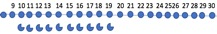
\includegraphics[width=3.0in]{figures/chordal_a_l.jpg}} 
  \hspace{1in} 
  \subfigure[Arrangement of agents at $T_{move\_{i+1}}$]{ 
    \label{fig:subfig:b} %% label for second subfigure 
    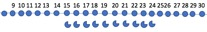
\includegraphics[width=3.0in]{figures/chordal_a1_l.jpg}}
  \caption{Arrangement of agents when moving} 
  \label{fig:subfig} %% label for entire figure 
\end{figure}

\noindent{\bf Three Jump NotificationTechnique}
In the model of BV decontamination exploring the network sequentially, explore agent moves forward for one step. If the node is safe, it move back to the leader agent, and then move forward to the safe node together. In this case, if the leader agent does not meet the leader in next $T$ after it moves forward, the leader agent learns that the original BV resides in the next node so it stop moving. 
But in our model, we employ $2d$ agents in the exploring phase, if they are not properly informed when one agent is destroyed by BV, in their next step of moving, some of them may be destroyed by the new formed BVs. In order to avoid the casualties, we propose $Three\,Jump\,Notification\,Technique$ to properly notice the agents who will move to the new formed BVs.
For convenience, let us take the node where the original BV resides as the original of the one-dimensional coordinate system. In a chordal ring $C_n(1, d_2, \ldots,  d_k)$, if the original BV is triggered, the clones of it spread to nodes whose coordinates are $-d_k$, $-d_{k-1}$, \ldots, $-d_2$, $-1$, $1$, $d_2$, \ldots, $d_{k-1}$, $d_k$. Obviously the nodes whose coordinates are $1$, $d_2$, \dots, $d_{k-1}$, $d_k$ may become the BV (Possible BV Nodes) now, our goal is to notify the agents which will move to these nodes to stop (Risky Agent). The coordinates of them are $1- d_k$, $d_2-d_k$, \ldots, $d_{k-1}-d_k$, $d_k-d_k$ (which is exactly the coordinate of the original BV) respectively. It is obvious that not all of the nodes from $1$ to $d_k$ become BV nodes after the triggering because there might be some agents already there, but since notifying all the $Risky\,Agents$(RAs) does not add more cost comparing to notifying some of them, in our strategy, we notify all of the RAs. Let us donate one of the Possible BV Nodes by $d_i$, and in our $ Three\,Jump\,Notification\,Technique$, agent residing in node $-d_i$ (Notification Agent) is employed to notify the agent residing in node $-d_k+\left |d_i\right |$ (RA) who will move to the BV node. 

We show that $Notification\,Agent$ are able to meet $Risky\,Agent$ in three steps: $-d_i\xrightarrow[]{move\left | d_i \right |}0\xrightarrow[]{move\,along\,chord\,k}-d_k\xrightarrow[]{move\,\left | d_i \right |}-d_k+\left|d_i\right|$. In this case, the notifying route of the $Notification\,\\Agent$ whose coordinate is $-d_k$ is $-d_k{\rightarrow}0{\rightarrow}-d_k{\rightarrow}0$ . We would make some modification in the $Surrounding\,and\,Elimination$ phase, but now let us assume it still follow the route above. The whole process of $Three\,Jump\,Notification\, Technique$ in chordal ring $C_n(1, 2, 4, 5)$ is shown in figure \ref{fig:tjt1, tjt2, tjt3, tjt4}. 

\begin{figure} [H]
  \centering 
  \subfigure[Arrangement of agents at $T_{move_i}$]{ 
    \label{fig:subfig:a} %% label for first subfigure 
    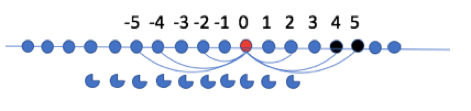
\includegraphics[width=2.5in]{figures/tjt1.png}} 
  \hspace{1in} 
  \subfigure[Arrangement of agents at $T_{notification_i}$]{ 
    \label{fig:subfig:b} %% label for second subfigure 
    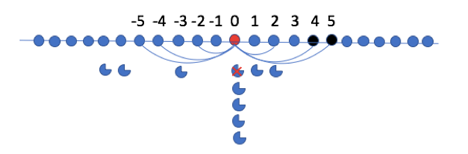
\includegraphics[width=2.5in]{figures/tjt2.png}} \
  \hspace{1in} 
  \subfigure[Arrangement of agents at $T_{notification_i'}$]{ 
    \label{fig:subfig:c} %% label for second subfigure 
    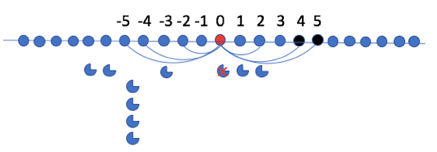
\includegraphics[width=2.5in]{figures/tjt3.png}} 
  \hspace{1in} 
  \subfigure[Arrangement of agents at $T_{notification_i''}$]{ 
    \label{fig:subfig:d} %% label for second subfigure 
    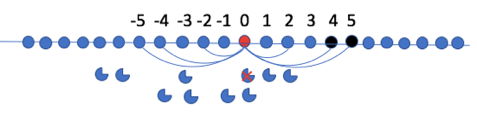
\includegraphics[width=2.5in]{figures/tjt4.png}} 
  \caption{The whole process of the Three Notifying Technique in chordal ring $C_n(1, 2, 4, 5)$} 
  \label{fig:subfig} %% label for entire figure 
\end{figure}

If the original BV residing in the red node, then once an agent moves to it, the agent and the BV are destroyed but the clones of the BV spread to all its neighbours. According to our technique, nodes whose coordinates are $1$, $2$, $4$, $5$ become $Possible\,BV\,Nodes$; agents residing in nodes $-4$, $-3$, $-1$, $0$ are the $Risky\, Agents$; agents residing in nodes $-5$, $-4$, $-2$, $-1$ are the $Notice\,Agents$. The routes for agents residing in nodes $-5$, $-4$, $-2$, $-1$ are $-5{\rightarrow}0{\rightarrow}-5{\rightarrow}0$; $-4{\rightarrow}0{\rightarrow}-5{\rightarrow}-1$; $-2{\rightarrow}0{\rightarrow}-5{\rightarrow}-3$; $-1{\rightarrow}0{\rightarrow}-5{\rightarrow}-4$ respectively.

\noindent{\bf Safe Exploring with Three Jump Notifying Technique}

After the initialization, agents employed in the first round move as the route we introduced in "Initialization" . When one of the agents is destroyed at $T-{move\_i}$, then $Three\,Jump\,Notification\,Technique$ begins. In "Route of the agent in exploring phase", we say that in the exploring phase every cycle contains one unit of time for moving and three units of time for notifying. Actually, the three units of time for notice are reserved for $Three\,Jump\, Notice\,Technique$, even though it only executes when one of the agents is destroyed. In another word, before encountering a BV, all the agents just stay where they are in the notice time.
After executing the $Three\,Jump\,Notice\,Technique$, the $Notice\,Agents$ move back to where they are before the notification. For example, in the example in "Three\,Jump\,Notification\,Technique", Notification Agent residing in node $-1$ moves back to node $-4$ following the reverse route in the notice phase which is $-1{\rightarrow}-5{\rightarrow}0{\rightarrow}-4$. 
 
\begin{theorem}
In the worst case scenario, the \bv is detected in $5n-9$ moves.
 
%When the BV is detected in the worst case scenario, three new black viruses are  triggered.
\end{theorem}
\begin{proof}
The worst case for the number of moves required occurs when the \bv  is found at node $v_i$, where $i=n-1$. 
%after exploring   $n-1$ nodes.  
  In this case, the $BV$ triggers no new \bvs since all the neighbours have already been explored in the safe area and are all protected by $SH$s.
%Note that  $LEA$ might  the $BV$ at the first node next to the home base, which would be the best case considering the number of moves for this phase (just one move made by $EA$).
% On the other hand, The worst case happens when $LEA$ and $EA$ pass through the whole outer ring nodes until reaching node $n-1$. 
% 
 The complexity of this case would be $(3(n-1)-2)$ for the movement of $LEA$ and $EA$, $(n-1-k)$ for one $SH$, $(n-1-p)$ for the second $SH$, $(k-1)$ for the third $SH$ and $(p-1)$ for the fourth $SH$ for a total $5n-9$ moves.
% and $1$ move to send a $CA$ to trigger the virus., I can't include one in here since I'm looking for the worst case in this phase, the CA's move would be part of phase 2.
\end{proof}
\begin{theorem}
In any triple loop chordal ring $C$, the worst case scenario in term of the number of agents required occurs when five new \bvs are created after triggering the original virus.
% $size(C)=8$ and $spread(C)=4$.
%When the \bv resides in node $v_i$, where $1 \leq i < k$, is considered , where 
%When  the BV is detected in the worst case 3 new BV are  triggered.
\end{theorem}

\begin{proof}
The worst case for the number of cleaning agents ($CA$) and surrounding agents ($SA$) occurs when the \bv is located at node $v_i$ where $1 \leq i < p$. In this case, where the \bv is $x_0$, it  triggers five new \bvs at $x_1$, $x_p$, $x_k$, $x_{-p}$ and $x_{-k}$ because no $SH$ have been deployed. $x_{-1} $ is always occupied by $LEA$. %The complexity of this case would be a maximum of $3p-5$ for the number of moves, $17$ $SA$s and $5$ $CA$s in addition to  $LEA$ and   $EA$.
% why did i write $3k+6$ for the number of moves
\end{proof}



\subsection{Surrounding and Eliminating}

 

In the triple loop chordal ring, when the \bv is triggered it may affect up to five  neighbouring nodes.
If $x_0$ is the original $BV$ node,, node $x_{-1}$ is always protected by $LEA$. $x_{1} $,$x_{p} $, $x_{k}$,$x_{-p} $ and $x_{-k}$ are  protected only if they belong to the safe area and are occupied by $SH$s.
To summarize, the best case scenario in terms of the number of  {\it black viruses}, after $EA$ triggers the original black virus, is that no more $BV$s are created, while the worst case scenario is that five $BV$s are created.  \\In order to handle the spread of $BV$s, the $LEA$ has to send agents to surround and clear those faults. 
%The distribution of agents can be done in a parallel or sequential manner. In the {\it Parallel distribution}, 
As with double loops, the $LEA$ creates $SA$(s) to be sent to specific targets, and when all agents are in position, the $LEA$ sends $CA$(s) to trigger all the $BV$s at the same time. Thus, we need as many $SA$s as the neighbours of the $BV$s and as many $CA$s as the $BV$s. 



For our convenience, we separated the topology into five segments, where the  \bv at ($v_i$) is located in one of those five segments as seen in figure \ref{fig:tloop-seg}.

\begin{figure} 
  \centering 
  \subfigure[Small Box with a Long Caption]{ 
    \label{fig:subfig:a} %% label for first subfigure 
    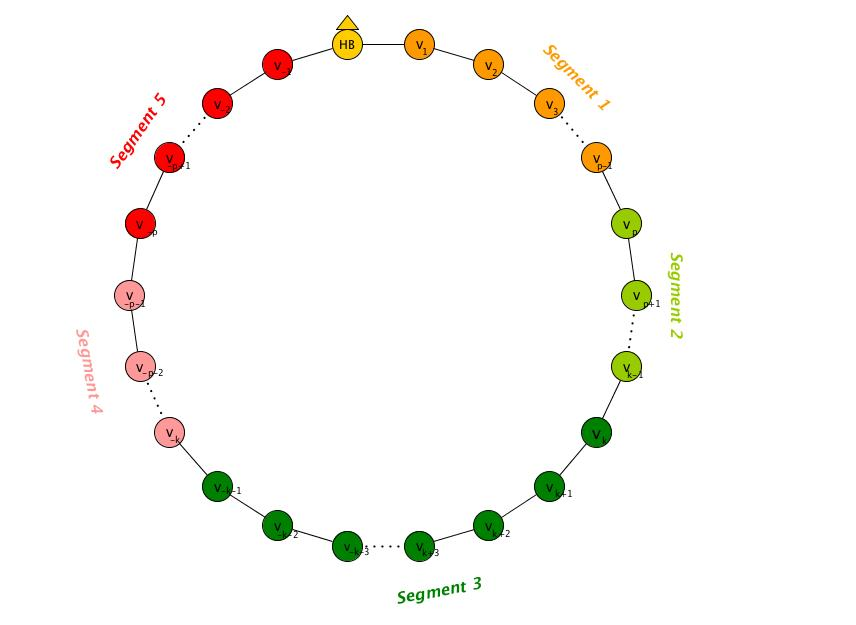
\includegraphics[width=1.5in]{figures/tloop_seg.jpg}} 
  \hspace{1in} 
  \subfigure[Big Box]{ 
    \label{fig:subfig:b} %% label for second subfigure 
    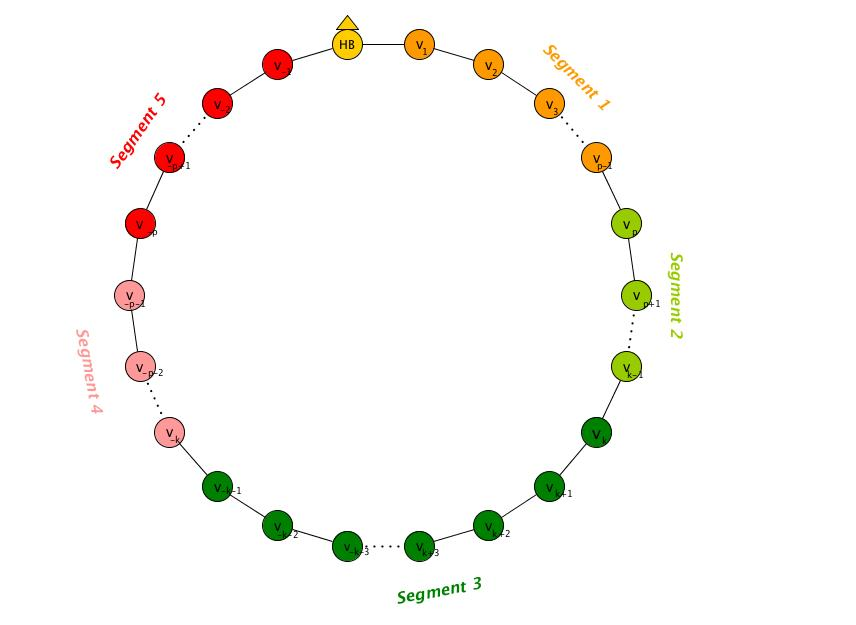
\includegraphics[width=1.5in]{figures/tloop_seg.jpg}} \
  \hspace{1in} 
  \subfigure[Big Box222]{ 
    \label{fig:subfig:b} %% label for second subfigure 
    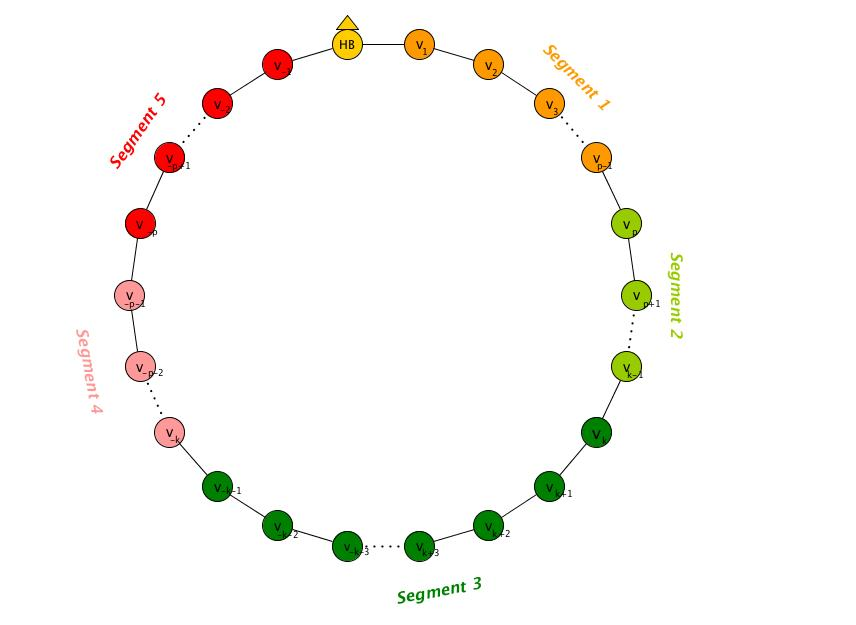
\includegraphics[width=1.5in]{figures/tloop_seg.jpg}} 
  \hspace{1in} 
  \subfigure[Big Box333]{ 
    \label{fig:subfig:b} %% label for second subfigure 
    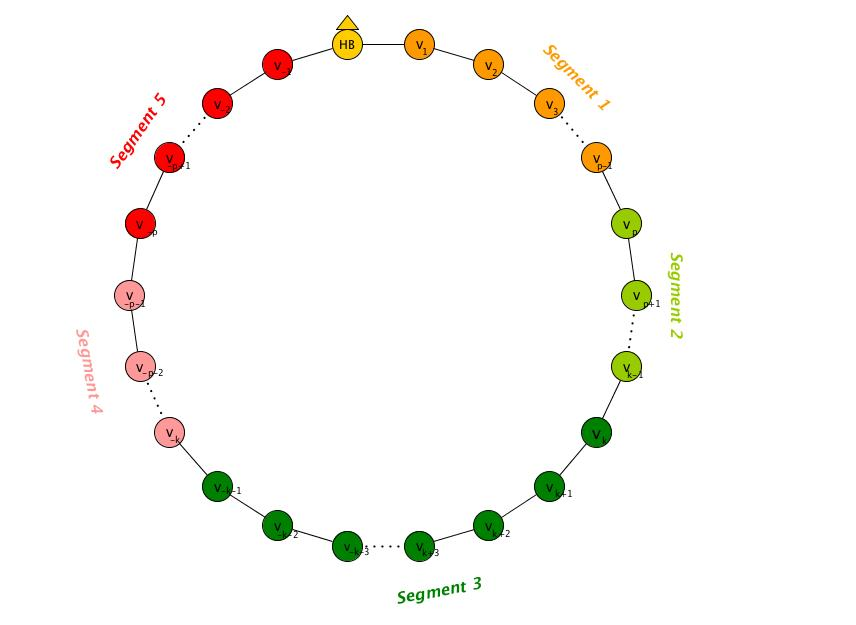
\includegraphics[width=1.5in]{figures/tloop_seg.jpg}} 
  \caption{Two Subfigures} 
  \label{fig:subfig} %% label for entire figure 
\end{figure}

\begin{figure}[H]
  \centering  
  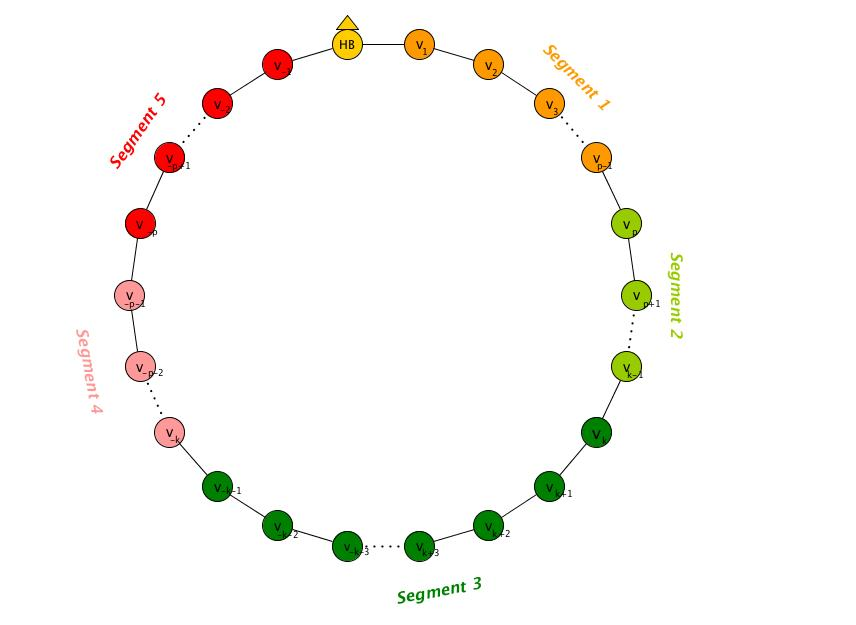
\includegraphics[width=0.6\textwidth]{figures/tloop_seg.jpg}
  \caption{Dividing the triple loop into five segments.}\label{fig:tloop-seg}
\end{figure}

\begin{itemize}

\item {\bf Segment 1:}  this segment contains nodes $v_1,v_2,...,v_{p-1}$ and the size of the safe area is $ |S_{area}| \leq p-1$.
\item {\bf Segment 2:}  this segment contains nodes $v_p,v_{p+1},...,v_{k-1}$ and the size of the safe area is $p \leq |S_{area}| \leq k-1$.
\item {\bf Segment 3:} this segment contains nodes $v_k,v_{k+1},...,v_{n-k-1}$ and the size of the safe area is $k \leq |S_{area}| \leq n-k-1$.
\item {\bf Segment 4:} this segment contains nodes $v_{n-k},v_{n-k+1},...,v_{n-p-1}$ and the size of the safe area is $n-k \leq |S_{area}| \leq n-p-1$.
\item {\bf Segment 5:}   this segment contains nodes $v_{n-p},v_{n-p+1},...,v_{n-1}$ and the size of the safe area is $n-p \leq |S_{area}| \leq n-1$.
\end{itemize}

%\end{proof}


The number of agents required to disinfect the triple loop chordal ring $C_n(1,p,k)$ is fixed regardless of  the surrounding strategy employed, whereas the number of moves necessary varies depending on the deployment method.


\begin{theorem}

Regardless of deployment strategy and chords length, a maximum of $24$ agents are employed  in   any   triple loop $C_n(1,p,k)$ for black virus disinfection.
\end{theorem}
\begin{proof}
The number of agents is determined by the location of the original $BV$, regardless of the deployment method. As previously mentioned, the \bv is found in one of five segments:
\begin{itemize} 
\item 
If the $BV$ is located at any node in {\em Segment 1}, we would have the worst complexity in terms of $CA$ and $SA$ since activating the \bv will create five more \bvs at $x_{1},x_{p},x_{k},x_{-p}$  and $x_{-k}$. In addition to the $LEA$ which is located at $x_{0}$, the $LEA$ deploys $17$  $SA$s to occupy $x_{2}$, $ x_{p-1}$,  $x_{k-1}$, $x_{p+1}$, $x_{k+1}$, $x_{k-p}$, $x_{k+p}$, $x_{2p}$, $x_{2k}$, $x_{-k+p}$, $x_{-p+1}$, $x_{-p-1}$, $x_{-k+1}$, $x_{-k-1}$, $x_{-k-p}$, $x_{-2p}$ and $x_{-2k}$. If the $BV$ is found in this segment, $Spread(C)=6$ and $Size(C)=24$.  
%If the $BV$ is located at any node in this segment, our team of agents consists of $24$ agents: $6$ $CA$s, $17$  $SA$s and $LEA$
 
\item If the $BV$ is located at any node in {\em Segment 2}, activating the original \bv would create four more \bvs at $x_{1},x_{p},x_{k}$ and $x_{-k}$ while $x_{-p}$ is guarded by a $SH$. In addition to the $SH$ at $x_{-p+1}$ and $LEA$ at $x_{-1}$, the $LEA$ deploys $14$  $SA$s to occupy $x_{2}$, $x_{p-1}$,  $x_{k-1}$, $x_{p+1}$, $x_{k+1}$, $x_{k-p}$, $x_{k+p}$, $x_{2p}$, $x_{2k}$, $x_{-k+p}$, $x_{-k+1}$, $x_{-k-1}$, $x_{-k-p}$ and$x_{-2k}$. If $BV$ is found in this segment, $Spread(C)=5$ and $Size(C)=21$.   
%If the $BV$ is located at any node in this segment, our team of agents consists of $22$ agents: $5$ $CA$s, $15$  $SA$s, $1$ $SH$ and $LEA$.

\item If the $BV$ is located at any node in {\em Segment 3}, activating the original \bv would create three more \bvs at $x_{1},x_{p}$ and $x_{k}$ while $x_{-p}$ and $x_{-k}$ are guarded by $SH$s. Therefore, in addition to the $SH$s at $x_{-p+1},x_{-k+1}$ and $LEA$ at $x_{0}$,the $LEA$ deploys $10$  $SA$s to occupy $x_{2}$, $x_{p-1}$, $x_{k-1}$, $x_{p+1}$, $x_{k+1}$, $x_{k-p}$, $x_{k+p}$, $x_{2p}$, $x_{2k}$ and $x_{p-k}$. If the $BV$ is found in this segment, $Spread(C)=4$ and $Size(C)=17$.   
%If the $BV$ is located at any node in this segment, our team of agents consists of $17$ agents: $4$ $CA$s, $10$  $SA$s, $2$ $SH$s and $LEA$.
 
\item {\em Segment 4} is part of the so called {\it Danger area} ($D_{area}$). Since our protocol is monotone, the explored nodes should be protected from reinfection; therefore, more $SH$(s) are deployed.  
If the $BV$ is located at any node in this segment, activating the original \bv would create two more \bvs at $x_{1}$ and $x_{p}$ while $x_{-p},x_{-k}$ and $x_{k}$ are guarded by $SH$s. Therefore, in addition to the $SH$s at $x_{-p+1},x_{-k+1},x_{k+1}$ and $LEA$ at $x_{0}$, the $LEA$ deploys $6$  $SA$s to occupy $x_{2}$, $x_{p-1}$, $x_{p+1}$, $x_{p-k}$, $x_{p+k}$ and $x_{2p}$. $Spread(C)=3$ and $Size(C)=13$.   
%If the $BV$ is located at any node in this segment, our team of agents consists of $13$ agents: $3$ $CA$s, $6$  $SA$s, $3$ $SH$s and $LEA$.

\item 
{\em Segment 5} is also a part of the {\it Danger area} ($D_{area}$) so more $SH$s are deployed in order to maintain the monotonicity of our protocol. This segment is divided into two cases:
\begin{itemize}
\item When $n-p\leq i < n-1$:

If the $BV$ is located at any node in this segment, activating the original \bv would create only one \bv at $x_{1}$, while $x_{-p},x_{-k},x_{k}$ and $x_{p}$ are guarded by $SH$s. Subsequently, in addition to the $SH$ at $x_{-p+1},x_{-k+1},x_{k+1},x_{p+1}$, and $LEA$ at $x_{0}$, the $LEA$ deploys $1$  $SA$ to occupy $x_{2}$. $Spread(C)=2$ and $Size(C)=8$.  
%If the $BV$ is located at any node in this segment, our team of agents consists of $8$ agents: $2$ $CA$s, $1$  $SA$, $4$ $SH$ and $LEA$.
\item  When $i=n-1$: 
In this case, no more \bvs are created since all neighbours are guarded by $SH$s and the $LEA$. No $SA$s are deployed and all the moves are done in the first phase. $Spread(C)=1$ and $Size(C)=7$.  
\end{itemize}
\end{itemize}
\end{proof}
%\begin{theorem}\label{no_greedy}
%For deploying surrounding agents in triple loop chordal rings, the simple greedy and the smart greedy strategies do not correctly perform the routing.
%\end{theorem}
%  \begin{proof}
%
%The greedy strategies would never do the routing in triple loop correctly because according to the chords structure, an agent could be caught  in an infinite loop. For example,  consider  a triple loop $C_n(1,2,k>9)$, with target  $x_{3}$. Starting from $x_{0}$, an agent would move greedily to $x_{-1}$ then to $x_{-2}$; when the agent reaches $x_{-2}$, it moves to the closest neighbour to $x_{3}$ excluding $x_{-1}$ and any infected neighbour, so it   moves to $x_{0}$ again which form an infinite loop. 
%By analogy with $t=x_{2}$, some other nodes would never be reached. 
%The greedy approach might work in some cases in triple loop rings especially if $p$ and $k$ are  relatively small values. Since we can not have all possible combinations of numbers $(p,k)$, we can generalize that the greedy strategies we proposed for routing in the double loop chordal rings can not be applied in triple loop chordal rings.
%\end{proof}

\subsubsection{\bf Greedy Deployment.}\label{no-greedy}



We noted that the greedy strategy could not be used for the deployment part of this phase, because, according to the chord structure, an agent could be caught  in an infinite loop. For example,  consider  a triple loop $C_n(1,2,k>9)$ with the target  $x_{3}$. Starting from $x_{0}$, an agent would move greedily to $x_{-1}$ then to $x_{-2}$; when the agent reached $x_{-2}$  it would move to the closest neighbour of  $x_{3}$, excluding $x_{-1}$ and any infected neighbour, thus moving to $x_{0}$ again and forming an infinite loop. 


As a result, we focus only on the non-local, move-optimal approach where optimal paths are computed by the $LEA$.
\subsubsection{\bf Move-Optimal Deployment.}
Due to the complexity of the chord structure, we can only provide an upper bound on the length of the optimal paths.
 
After triggering the original $BV$, which is $x_{0}$,  the neighbouring nodes are in one of two states: guarded or contaminated.
Node $x_{-1}$ is  guarded by $LEA$. Nodes $x_{1}$, $x_{p}$, $x_{k}$, $x_{-p}$ and $x_{-k}$ could be in either state depending on the size of the {\it safe area}.
All possible targets in the worst case scenario are: ${\cal T}$=$\{x_{2}$, $x_{p-1}$, $x_{p-k}$, $x_{k-1}$, $x_{p+1}$, $x_{k+1}$, $x_{k-p}$, $x_{k+p}$, $x_{2p}$, $x_{2k}$, $x_{-p+1}$, $x_{-p-1}$, $x_{-k+1}$, $x_{-k-1}$, $x_{-k-p}$, $x_{-2p}$, $x_{-2k}\}$. In fact, sometimes some of these targets could be $BV$s or common neighbours depending on the structure of the chordal ring. 



We now specify a path for each target, the length of which is certainly an upper bound of the optimal path length. In this type of chordal ring, the length of these paths is constant, regardless of the target. As we did for the double loop, we have listed the special paths $\sigma_i$ below.




 
\begin{center}
  \begin{tabular}{|c|l|}
 \hline
 Target $x_i$ & Special Path $\sigma_i$\\
 \hline
  $x_{2}$ &  $ x_{0} \xrightarrow {-1} x_{-1} \xrightarrow {+k} x_{k-1} \xrightarrow {+k} x_{2k-1} \xrightarrow {+1} x_{2k}  \xrightarrow {+1} x_{2k+1} \xrightarrow {+1} x_{2k+2} \xrightarrow {-k} x_{k+2} \xrightarrow {-k} x_{2}$\\
  $x_{p-1}$ &  $ x_{0} \xrightarrow {-1} x_{-1} \xrightarrow {+p} x_{p-1} $\\
  $x_{k-1}$ &  $ x_{0} \xrightarrow {-1} x_{-1} \xrightarrow {+k} x_{k-1} $\\
  $x_{p-k}$ &  $ x_{0} \xrightarrow {-1} x_{-1} \xrightarrow {+p} x_{p-1} \xrightarrow {-k} x_{-k+p-1} \xrightarrow {+1} x_{p-k}$\\
  $x_{p+1}$ &  $ x_{0} \xrightarrow {-1} x_{-1} \xrightarrow {+p} x_{p-1}\xrightarrow {+p} x_{2p-1}\xrightarrow {+1} x_{2p} \xrightarrow {+1} x_{2p+1}\xrightarrow {-p} x_{p+1}$\\
  $x_{k+1}$ &  $\ x_{0} \xrightarrow {-1} x_{-1} \xrightarrow {+k} x_{k-1}\xrightarrow {+k} x_{2k-1}\xrightarrow {+1} x_{2k} \xrightarrow {+1} x_{2k+1}\xrightarrow {-p} x_{k+1}$\\
  $x_{k-p}$ &  $ x_{0} \xrightarrow {-1} x_{-1} \xrightarrow {+k} x_{k-1} \xrightarrow {-p} x_{k-p-1}\xrightarrow {+1} x_ {k-p}$\\

$x_{k+p}$ &   $ x_{0}\xrightarrow {-1} x_{-1} \xrightarrow {+p} x_{p-1} \xrightarrow {+k} x_{k+p-1} \xrightarrow {+1} x_{k+p}$\\
  $x_{2p}$ &  $ x_{0} \xrightarrow {-1} x_{-1} \xrightarrow {+p} x_{p-1} \xrightarrow {+p} x_{2p-1}\xrightarrow {+1} x_{2p}$\\
  $x_{2k}$ &  $ x_{0} \xrightarrow {-1} x_{-1} \xrightarrow {+k} x_{k-1} \xrightarrow {+k} x_{2k-1}\xrightarrow {+1} x_{2k}$\\
 $x_{-p+1}$ & $ x_{0} \xrightarrow {-1} x_{-1} \xrightarrow {-p} x_{-p-1} \xrightarrow {-p} x_{-2p-1} \xrightarrow {+1} x_ {-2p} \xrightarrow {+1} x_ {-2p+1}\xrightarrow {+p} x_ {-p+1}$\\
 $x_{-k+1}$ & $ x_{0} \xrightarrow {-1} x_{-1} \xrightarrow {-k} x_{-k-1} \xrightarrow {-k} x_{-2k-1} \xrightarrow {+1} x_ {-2k} \xrightarrow {+1} x_ {-2k+1}\xrightarrow {+k} x_ {-k+1}$\\
 $x_{-p-1}$ & $ x_{0} \xrightarrow {-1} x_{-1} \xrightarrow {-p} x_{-p-1} $\\
 $x_{-k-1}$ & $ x_{0} \xrightarrow {-1} x_{-1} \xrightarrow {-k} x_{-k-1} $\\

 $x_{-k-p}$  & $ x_{0} \xrightarrow {-1} x_{-1} \xrightarrow {-k} x_{-k-1} \xrightarrow {-p} x_{-k-p-1}\xrightarrow {+1} x_{-k-p} $\\

$x_{-2p}$  & $ x_{0} \xrightarrow {-1} x_{-1} \xrightarrow {-p} x_{-p-1} \xrightarrow {-p} x_{-2p-1}\xrightarrow {+1} x_{-2p} $\\
$x_{-2k}$  & $ x_{0} \xrightarrow {-1} x_{-1} \xrightarrow {-k} x_{-k-1} \xrightarrow {-k} x_{-2k-1}\xrightarrow {+1} x_{-2k} $\\

 \hline
 \end{tabular}
 \end{center}

Depending on the chords structure, shorter paths can be devised in some cases. A detailed analysis of all possible situations is carried out in Appendix \ref{AppendixA}.
 

The following table summarizes the upper bound of  the number of moves required to reach each possible target. Notice that we distinguish between two situations: when $\left\vert{S_{area}}\right\vert < p$ and  when $\left\vert{S_{area}}\right\vert \ge k$. The former situation represents the worst possible number of \bvs while the latter situation combines different cases where the number of \bvs decreases according to the location of the original {\it black virus}.
\begin{center}
\begin{tabular}{|l|lr|lr|}\hline
\multirow{2}{1 in}{Destination} &
\multicolumn{2}{c|}{Number of moves}
\\
& $\left\vert{S_{area}}\right\vert < p$ & $\left\vert{S_{area}}\right\vert \ge k$ \\\hline\hline
$x_0$       & $1$ & $1$  \\\hline
$x_2$       & $\leq8$ & $\leq 4$  \\\hline
$x_{p-1}$    & $2$   & $2$     \\\hline
$x_{k-1}$    & $2$   & $2$     \\\hline
$x_{p+1}$ & $\leq 6$   & $\leq 4$         \\\hline
$x_{k+1}$ & $\leq 6$   & $\leq 6$         \\\hline
$x_{k-p}$ & $\leq 4$   & $\leq 4$         \\\hline
$x_{k+p}$ & $\leq 4$   & $\leq 4$         \\\hline
$x_{2p}$            & $\leq 4$   & $\leq 4$        \\\hline
$x_{2k}$            & $ 4$   & $ 4$        \\\hline
$x_{-p+1}$    & $\leq 6$   & 1    \\\hline
$x_{-p-1}$    & $2$   & -     \\\hline
$x_{-2p}$ & $4$   & -        \\\hline
$x_{p-k}$            & $\leq 4$   & $\leq 4$        \\\hline
$x_{-k+1}$            & $\leq 6$   & $1$        \\\hline
$x_{-k-1}$    & $2$   & -     \\\hline
$x_{-k-p}$            & $4$   & -        \\\hline
$x_{-2k}$ & $4$   & -        \\\hline

$x_1$       & $1$ & $1$  \\\hline
$x_p$       & $1$ & $1$  \\\hline
$x_k$       & $1$ & $1$  \\\hline
$x_{-p}$       & $1$ & -  \\\hline
$x_{-k}$       & $1$ & -  \\\hline
{\bf Total}     & $\leq 78$   & $\leq 44$ \\\hline
\end{tabular}
\captionof{table}{Move complexity  in shortly-chorded triple loops.}
\end{center}




 
 \begin{theorem}
In any triple loop   $C_n(1,p,k)$ where $\left\vert{S_{area}}\right\vert \ge k$, the number of moves required to surround and eliminate $BV$s is $\leq44$.
\end{theorem}
 \begin{proof}
In any triple loop chordal ring where $\left\vert{S_{area}}\right\vert \ge k$, the maximum number of moves required to reach all targets is $44$: One move is done by the $LEA$ to reach $x_0$. Node $x_{2}$ is reached within four moves.
 Node $x_{p-1}$ is reached within two moves.
 Node $x_{k-1}$ is reached within two moves.
 Node $x_{p+1}$ is reached within four moves.
 Node $x_{k+1}$ is reached within six moves.
 Node $x_{k-p}$ is reached within four moves.
  Node $x_{k+p}$ is reached within four moves.
 Node $x_{2p}$ is reached within four moves.
 Node $x_{2k}$ is reached within four moves.
 Node $x_{p-k}$ is reached within four moves.
 Two moves are made by the $SH$s in order to move from $x_{-p}$ and $x_{-k}$ to $x_{-p+1}$ and $x_{-k+1}$  when they receive copies of the original $BV$.
 After all of the agents arrive at their destinations the $LEA$ sends three $CA$s to the \bvs at $x_{1}$, $x_{p}$ and $x_{k}$ in three moves. Notice that since we always compare the resulting routes $\pi_z$, where $z \in \mathbb{Z}$  to the  $\sigma_i$, none of $\pi_z$ would be greater than the corresponding $\sigma_i$. 
\end{proof}

\begin{theorem}
In any triple loop   $C_n(1,p,k)$ where $\left\vert{S_{area}}\right\vert < p$, the number of moves required to surround and eliminate the $BV$s is $\leq78$.
\end{theorem}
 \begin{proof}
In any triple loop chordal ring where $\left\vert{S_{area}}\right\vert <p$, the maximum number of moves required to reach all targets is $78$. One move is made by the $LEA$ to reach $x_0$.
 Node $x_{2}$ is reached within eight moves.
 Node $x_{p-1}$ is reached within two moves.
 Node $x_{k-1}$ is reached within two moves.
 Node $x_{p+1}$ is reached  within six moves.
 Node $x_{k+1}$ is reached within six moves.
 Node $x_{k-p}$ is reached within four moves.
 Node $x_{k+p}$ is reached within four moves.
 Node $x_{2p}$ is reached within four moves.
 Node $x_{2k}$ is reached within four moves.
 Node $x_{-p+1}$ is reached within six moves.
 Node $x_{-p-1}$ is reached within two moves.
 Node $x_{-2p}$ is reached within four moves.
 Node $x_{p-k}$ is reached  within four moves.
 Node $x_{-k+1}$ is reached within six moves.
 Node $x_{-k-1}$ is reached within two moves.
 Node $x_{-k-p}$ is reached within four moves.
 Node $x_{-2k}$ is reached within four moves.
 After all agents arrive at their destinations the $LEA$ sends five $CA$s to the \bvs at $x_{1}$, $x_{p}$, $x_{k}$,$x_{-p}$ and $x_{-k}$ in five moves. Notice that since we always compare the resulting routes $\pi_z$, where $z \in \mathbb{Z}$  to the  $\sigma_i$, none of $\pi_z$ would be greater than the corresponding $\sigma_i$. 
\end{proof}


 %{\bf Discussion on Optimality.}
%In triple loops, we can not claim that {\em Move-optimal} strategy we discussed above provides optimal routes since it is difficult to consider all possible combinations of the numbers $p$ and $k$. However, we have an upper bound number of moves to reach each target $x_i$ which corresponds to $\sigma_i$.



%It requires the same number of agents, casualties, and moves as the aforementioned Move-optimal algorithm.
%#####################################################################


 In the following two sections we will investigate the black virus disinfection problem in  triple loop chordal rings for the two extreme cases previously mentioned. In these cases we can derive an exact bound on the optimal path lengths.




\section{Triple Loops: the Case of $C_n(1,2,k)$ }
\subsection{Exploring and Shadowing}
As we explained earlier, this phase is common to all chordal rings. We instantiate it below for the particular case of   $C_n(1,2,k)$.
%\begin{comment}
%The two agents  $LEA$ and $EA$   explore each node on the outer ring in a clockwise direction starting from the homebase  using the {\em safe exploration} technique:  $LEA$ and$EA$ are at node $v_{j}$, $EA$ moves to the next node $v_{j+1}$ while $LEA$ waits at $v_{j}$; if $EA$ returns back to its leader, they both move to $v_{j+1}$, otherwise, the $BV$ is detected and $EA$ is destroyed. 
%In order to diminish the effect of the $BV$,  shadow agents are deployed to guard the explored neighbours of the next node to be visited; However, this can not be happening unless $LEA$ and $EA$ have passed through at least $p$ nodes. In other words, if  $|S_{area}|\ge p$. 
%
%As we discussed in \ref{monotone_ph1},  this phase correctly locates the original  \bv and it is monotone since the maximum number of $SH$s recruited from the beginning is $5$ (i.e., as many as the number of neighbours in the worst case $v=n-1$).
%  \end{comment}


 \begin{center}
\fbox{
\begin{minipage}{6cm}
{\sc  Exploring and Shadowing}

  \begin{tabbing}
let $HB= v_0$ \\
  Age\= nts $EA $ and $$LEA$$ at safe node  $v_i$.\\ \\

if ($ i =0$)\\
\>   $N_{ex}(v_{i+1}) = \{ v_{0}\}$ \\
\>   no $SH$ has been deployed  \\ 

if ($2 \leq i+1 < k$)\\
\>   $N_{ex}(v_{i+1}) = \{ v_{i-1},v_{i} \}$ \\
\>  1 $SH$ has been deployed to protect $v_{i-1}$\\ 

if ($k \leq i+1 < n-k$)\\
\>   $N_{ex}(v_{i+1}) = \{ v_{i},v_{i-1},v_{i+1-k} \}$ \\
\>  2 $SH$s have been deployed to protect $v_{i-1},v_{i+1-k}$\\ 

if ($n-k \leq i+1 < n-2$)\\
\>   $N_{ex}(v_{i+1}) = \{ v_{i},v_{i-1},v_{i+1-k},v_{i+1+k} \}$ \\
\>  3 $SH$s have been deployed to protect $v_{i-1},v_{i+1-k},v_{i+1+k}$\\ 

if ($ i = n-3$)\\
\>   $N_{ex}(v_{i+1}) = \{ v_{i},v_{i-1},v_{i+1-k},v_{i+1+k},v_{0} \}$ \\
\>  $4$ $SH$s have been deployed to protect $v_{i-1},v_{i+1-k},v_{i+1+k},v_{0}$\\ 


if ($i = n-2$)\\
\>   $N_{ex}(v_{i+1}) =  \{ v_{i},v_{i-1},v_{i+1-k},v_{i+1+k},v_{1},v_{0} \}$ \\
\>  $5$ $SH$s have been deployed to protect $v_{i-1},v_{i+1-k},v_{i+1+k},v_{1},v_{0}$\\ \\
 EA moves to $v_{i+1}$.\\ 
 \end{tabbing}
\end{minipage}
}
\end{center}

\noindent The observations below were made following the employment of this strategy:

\begin{theorem}
In the worst case scenario, the \bv is detected using $5n-9$ moves.
 
%When  the BV is detected in the worst case 3 new BV are  triggered.
\end{theorem}
\begin{proof}
The worst case scenario for the number of moves required occurs when the \bv  is found at node $v_i$, where $i=n-1$. 
%after exploring   $n-1$ nodes.  
  In this case the $BV$ triggers no new \bvs since all  of the neighbouring nodes in the safe area have been explored and all are protected by $SH$s.
%Note that  $LEA$ might  the $BV$ at the first node next to the home base, which would be the best case considering the number of moves for this phase (just one move made by $EA$).
% On the other hand, The worst case happens when $LEA$ and $EA$ pass through the whole outer ring nodes until reaching node $n-1$. 
% 
 The complexity of this case would be $(3(n-1)-2)$ for the movement of $LEA$ and $EA$, $(n-1-k)$ for one $SH$ to guard node $v_{n-1-k}$, $(n-3)$ for the second $SH$ to guard node $v_{n-3}$, $(k-1)$ for the third $SH$ to guard node $v_{k-1}$ and $(1)$ for the fourth $SH$ to guard node $v_{1}$ for a total of $5n-9$ moves.
% and $1$ move to send a $CA$ to trigger the virus., I can't include one in here since I'm looking for the worst case in this phase, the CA's move would be part of phase 2.
\end{proof}
\begin{theorem}
In any triple loop chordal ring $C_n=\{1,2,k\}$, the worst case scenario in terms of the number of agents required occurs when five new \bvs are created after triggering the original virus.
% $size(C)=8$ and $spread(C)=4$.
%When the \bv resides in node $v_i$, where $1 \leq i < k$, is considered , where 
%When  the BV is detected in the worst case 3 new BV are  triggered.
\end{theorem}
\begin{proof}
The worst case scenario in terms of the number of cleaning agents ($CA$s) and surrounding agents ($SA$s) occurs when the \bv is at node $v_i$ where $ i =1$. In this case, where the \bv is $x_0$, it  triggers five new \bvs at $x_1$, $x_2$, $x_k$, $x_{-2}$ and $x_{-k}$ because no $SH$ have been deployed. Note that  $x_{-1} $ is always occupied by $LEA$. In this case, the maximum number of  \bvs would be created.
%, $15$ $SA$s and $5$ $CA$s in addition to $LEA$ and $EA$.
% why did i write $3k+6$ for the number of moves
\end{proof}



\subsection{Surrounding and Eliminating}

As with the general case, in this class of triple loops, when the \bv is triggered it has the potential to affect up to five of its  neighbours by the end of the first phase. In the second phase, the $LEA$ creates $SA$(s) to be sent to specific targets and then sends $CA$(s) to activate all the \bvs at the same time and disinfect the entire topology.
\begin{comment}
 Let $x_0$ be the original $BV$, node $x_{-1}$ is always protected by $LEA$. $x_{1} $,$x_{2} $, $x_{k}$,$x_{-2} $, $x_{-k}$ are  protected only if they belong to the safe area and are occupied by $SH$s; otherwise, they are affected depending on their location.
Summarizing, in the best case in term of the number of {\it black viruses}, after $EA$ triggers the original black virus, no more $BV$s are created, while the worst case, five $BV$s are created.  \\
To handle the spread of the $BV$s, $LEA$ has to send agents to surround and clear those faults. 
%The distribution of gents can be done in a parallel or sequential manner. In the {\it Parallel distribution}, 
To do so, $LEA$ creates $SA$(s) to be sent to specific targets, and after all agents are at their positions, $LEA$ sends $CA$(s) to trigger all the $BV$s at once, so we need as many $SA$s as the neighbours of the $BV$s, and as many $CA$s as the $BV$s. 


First, we remind some notation.   
Let $x_0$ be the discovered $BV$.
Let $V$ be  the set of all vertices. We denote by  ${\cal BV}$ the set of black viruses in the system.
 Let ${\cal S} = V - {\cal BV}$ be  the set of the  clean nodes not containing any $BV$. Let 
  ${\cal T}$ be  the set of targets, that is the nodes to be occupied. Let $S_{area}$ be the {\it safe area}, and  $\left\vert{S_{area}}\right\vert$ is the number of nodes in that area.  Let $D_{area}$ be the {\it danger area} where recontamination need to be avoided.
\end{comment}


  \begin{center}
\fbox{
\begin{minipage}{7.5cm}
{\sc Surrounding and Eliminating} 
  \begin{tabbing}
   $$LEA$$ \= and  $SH$s  covering all $N_{ex}(v)$ \\


if ($|S_{area}|=1$)( *$$LEA$$ is covering $x_{-1}$*) \\

  \tab   $N_{un}(x_0) =\{x_{1},x_{2},x_{k},x_{-2},x_{-k} \}$ \\ 


 if ($2\leq |S_{area}|<k$)(*$$LEA$$ and  $SH$  covering $x_{-1},x_{-2}$*)\\

  \tab   $N_{un}(x_0) =\{x_{1},x_{2},x_{k},x_{-k} \}$ \\ 

if  ($k\leq |S_{area}| <n-k$)(*$$LEA$$ \= and  2 $SH$s  covering $x_{-1},x_{-2},x_{-k}$*) \\


  \tab  $N_{un}(x_0) =\{x_{1},x_{2},x_{k}\}$  \\ 

if  ($n-k\leq |S_{area}| <n-2$)(*$$LEA$$ \= and  $SH$s  covering $x_{-1},x_{-2},x_{-k},x_{k}$*) \\

  \tab  $N_{un}(x_0) =\{x_{1},x_{2},\}$  \\ 

if  ($|S_{area}| =n-2$)(*$$LEA$$ \= and  $SH$s  covering $x_{-1},x_{-2},x_{-k},x_{k},x_{2}$*) \\

  \tab  $N_{un}(x_0) =\{x_{1}\}$  \\ 


Else (*$$LEA$$ \= and  $SH$s  covering $x_{-1},x_{-2},x_{-k},x_{k},x_{2},x_1$*) \\
  \tab  $N_{un}(x_0) =\emptyset $ \\ \\

  
 All $SH$ make one move in the clockwise direction.\\ %when they receive bv, they make 1 move and  stay there
 For \= each $u \in   N_{un}(x_0)$:\\
\>  {\sc Deploy}  an  agent   to each  $z\in \{N(u)\setminus  N_{un}(x_0)\}$\\

  Wh\=en $N(u)$ is covered:\\
 \> {\sc Deploy} one agent to   $u$
  \end{tabbing}
\end{minipage}
}
\end{center}




The exploring team will find the \bv at ($v_i$), which is located in one of the five segments of the chordal ring:
\begin{itemize}

\item {\bf Segment 1}: this segment contains node $v_1$ and the size of the safe area is $|S_{area}| =1$.
\item {\bf Segment 2}: this segment contains nodes $v_2,v_3,...,v_{k-1}$ and the size of the safe area is $2\leq |S_{area}| \leq k-1$.
\item {\bf Segment 3}: this segment contains nodes $v_k,v_{k+1},...,v_{n-k-1}$ and the size of the safe area is $k\leq |S_{area}| \leq n-k-1$.
\item {\bf Segment 4}: this segment contains nodes $v_{n-k},v_{n-k+1},...,v_{n-3}$ and the size of the safe area is $n-k\leq |S_{area}| \leq n-3$.
\item {\bf Segment 5}: this segment contains nodes $v_{n-2}$ and $v_{n-1}$ and the size of the safe area is $n-2 \leq|S_{area}| \leq n-1$.
\end{itemize}


%\end{proof}



The number of agents required to disinfect the triple loop chordal ring($C_n(1,2,k)$) is fixed, regardless of the surrounding strategy, whereas the number of moves varies depending on the deployment method.


\begin{theorem}


Regardless of the deployment strategy, a maximum of 22 agents are employed in any triple loop $C_n(1,2,k)$ for black virus disinfection.
\end{theorem}
\begin{proof}
The number of agents required  is determined by the location of the original $BV$, regardless of the deployment method.
\begin{itemize} 
\item If  the $BV$ is found in {\em Segment 1} we would have the worst complexity in terms of $CA$s and $SA$s since activating the \bv will create five more \bvs at $x_{1},x_{2},x_{k},x_{-2}$ and $x_{-k}$. In addition to the $LEA$ which is at $x_{0}$, the $LEA$ deploys $15$  $SA$s to occupy $x_{-1}$, $ x_{3}$,  $x_{4}$, $x_{k-2}$, $x_{k-1}$, $x_{k+1}$, $x_{k+2}$, $x_{2k}$, $x_{-3}$, $x_{-4}$, $x_{-k+1}$, $x_{-k+2}$, $x_{-k-1}$, $x_{-k-2}$ and $x_{-2k}$. Therefore, $Spread(C)=6$ and $Size(C)=22$.  
%If the $BV$ is located at any node in this segment, our team of agents consists of $22$ agents: $6$ $CA$s, $15$  $SA$s, and $LEA$
 
\item If the $BV$ is found in {\em Segment 2}, activating the original \bv would create four more \bvs at $x_{1},x_{2},x_{k}$ and $x_{-k}$ while $x_{-2}$ is guarded by a $SH$. In addition to the $SH$ at $x_{-1}$ and $LEA$ at $x_{0}$, the $LEA$ deploys $12$  $SA$s to occupy  $ x_{3}$,  $x_{4}$, $x_{k-2}$, $x_{k-1}$, $x_{k+1}$, $x_{k+2}$, $x_{2k}$, $x_{-k+1}$, $x_{-k+2}$, $x_{-k-1}$, $x_{-k-2}$ and $x_{-2k}$. Therefore, $Spread(C)=5$ and $Size(C)=19$.   
%If the $BV$ is located at any node in this segment, our team of agents consists of $19$ agents: $5$ $CA$s, $12$  $SA$s, $1$ $SH$ and $LEA$.

\item If the $BV$ is found in {\em Segment 3}, activating the original \bv would create three more \bvs at $x_{1},x_{2}$ and $x_{k}$ while $x_{-2}$ and $x_{-k}$ are guarded by $SH$s. Therefore, in addition to the $SH$s at $x_{-1}$ and $x_{-k+1}$ and $LEA$ at $x_{0}$, the $LEA$ deploys $8$  $SA$s to occupy  $ x_{3}$,  $x_{4}$, $x_{k-2}$, $x_{k-1}$, $x_{k+1}$, $x_{k+2}$, $x_{2k}$ and $x_{-k+2}$. Therefore, $Spread(C)=4$ and $Size(C)=15$.   
%If the $BV$ is located at any node in this segment, our team of agents consists of $15$ agents: $4$ $CA$s, $8$  $SA$s, $2$ $SH$s, and $LEA$.
 
\item If  the $BV$ is found in {\em Segment 4}, activating the original \bv would create two more \bvs at $x_{1}$ and $x_{2}$ while $x_{-2},x_{-k}$ and $x_{k}$ are guarded by $SH$s. Therefore, in addition to the $SH$s at $x_{-1},x_{-k+1}$ and $x_{k+1}$ and $LEA$ at $x_{0}$, the $LEA$ deploys $4$  $SA$s to occupy  $x_{3}$, $x_{4}$ $x_{-k+2}$ and $x_{k+2}$.  Therefore, $Spread(C)=3$ and $Size(C)=11$.   
%If the $BV$ is located at any node in this segment, our team of agents consists of $11$ agents: $3$ $CA$s, $4$  $SA$s, $3$ $SH$s, and $LEA$.

\item If the $BV$ is found in {\em Segment 5}, we have two possible cases:


\begin{itemize}
\item When $ i = n-2$:

If the $BV$ is located at  node $v_{n-2}$, activating the original \bv would create only one \bv at $x_{1}$, while $x_{-2},x_{-k},x_{k}$ and $x_{2}$ are guarded by $SH$s. Subsequently, in addition to the $SH$ at $x_{-1},x_{-k+1},x_{k+1},x_{3}$ and $LEA$ at $x_{0}$, the $LEA$ deploys $1$  $SA$ to occupy $x_{2}$. Therefore, $Spread(C)=2$ and $Size(C)=8$.
%If the $BV$ is located at any node in this segment, our team of agents consists of $8$ agents: $2$ $CA$s, $1$  $SA$, $4$ $SH$, and $LEA$.

\item  When $i=n-1$: %here \\
 
In this case, no more \bvs are created since all the neighbouring nodes are guarded by $SH$s and the $LEA$. No $SA$s need to be deployed and all the moves are made in the first phase. Therefore, $Spread(C)=1$ and $Size(C)=7$.  
%In this case,  the team consists of $7$ agents: $1$ $CA$, $5$ $SH$s, and $LEA$. 
\end{itemize}
\end{itemize}
\end{proof}

For the deployment part of this phase, we have demonstrated that a local greedy approach does not yield correct results, see \ref{no-greedy}. In the following section we discuss the non-local surrounding strategy in which  $SA$s follow  specific paths set up by the $LEA$ which has  knowledge of the topology.



\subsubsection{Move-Optimal Deployment}
As with the general triple loop, for the surrounding phase we specify each path for each target. Let us now consider all of the possible targets: ${\cal T}$=$\{x_{-1}$, $ x_{3}$,  $x_{4}$, $x_{k-2}$, $x_{k-1}$, $x_{k+1}$, $x_{k+2}$, $x_{2k}$, $x_{-3}$, $x_{-4}$, $x_{-k+1}$, $x_{-k+2}$, $x_{-k-1}$, $x_{-k-2}$, $x_{-2k}\}$.  The  special paths ($\sigma_i$) for this type of triple loop are described below. 

 
 
\begin{center}
  \begin{tabular}{|c|l|}
 \hline
 Target $x_i$ & Special Path $\sigma_i$\\
 \hline
  $x_{-1}$ &  $x_{0}\xrightarrow {-1} x_{-1}$\\
  $x_{k-1}$ &  $x_{0}\xrightarrow {-1}x_{-1}\xrightarrow {+k}x_{k-1}$\\
  $x_{k-2}$ &  $x_{0} \xrightarrow {-1}x_{-1}\xrightarrow {+k}x_{k-1}\xrightarrow {-1}x_{k-2}$\\
  $x_{k+1}$ &  $x_{0} \xrightarrow {-1}x_{-1}\xrightarrow {+k}x_{k-1}\xrightarrow {+2}x_{k+1}$\\
  $x_{k+2}$ &  $x_{0} \xrightarrow {-1}x_{-1}\xrightarrow {+k}x_{k-1}\xrightarrow {+2}x_{k+1}\xrightarrow {+1}x_{k+2}$\\
  $x_{3}$ &  $x_{0} \xrightarrow {-1}x_{-1}\xrightarrow {+k}x_{k-1}\xrightarrow {+2}x_{k+1}\xrightarrow {+2}x_{k+3}\xrightarrow {-k}x_{3}$\\
  $x_{4}$ &  $x_{0} \xrightarrow {-1}x_{-1}\xrightarrow {+k}x_{k-1}\xrightarrow {+2}x_{k+1}\xrightarrow {+2}x_{k+3}\xrightarrow {+1}x_{k+4} \xrightarrow {-k}x_{4}$\\

$x_{2k}$ &   $ x_{0} \xrightarrow {-1} x_{-1} \xrightarrow {+k} x_{k-1} \xrightarrow {+k} x_{2k-1} \xrightarrow {+1}  x_{2k}$\\
  $x_{-3}$ &  $x_{0}\xrightarrow {-1}x_{-1}\xrightarrow {-2}x_{-3}$\\
  $x_{-4}$ &  $x_{0}\xrightarrow {-1}x_{-1}\xrightarrow {-2}x_{-3} \xrightarrow {-1}x_{-4}$\\
 $x_{-k-1}$ & $ x_{0} \xrightarrow {-1} x_{-1} \xrightarrow {-k} x_{-k-1}$\\
 $x_{-k-2}$ & $ x_{0} \xrightarrow {-1} x_{-1} \xrightarrow {-k} x_{-k-1} \xrightarrow {-1} x_{-k-2}$\\
 $x_{-k+1}$ & $ x_{0} \xrightarrow {-1} x_{-1} \xrightarrow {-k} x_{-k-1} \xrightarrow {+2} x_{-k+1}$\\
 $x_{-k+2}$ & $ x_{0} \xrightarrow {-1} x_{-1} \xrightarrow {-k} x_{-k-1} \xrightarrow {+2} x_{-k+1}\xrightarrow {+1} x_{-k+2}$\\

 $x_{-2k}$  & $x_{0} \xrightarrow {-1} x_{-1} \xrightarrow {-k} x_{-k-1} \xrightarrow {-k} x_{-2k-1} \xrightarrow {+1} x_{-2k}$\\
 \hline
 \end{tabular}
 \end{center}
 
 \noindent Depending on the chords structure,  shorter paths could be devised in some cases. A detailed analysis of all the possible situations is carried out in the following discussion.

Let us now consider the different routes to each target in six different cases, depending on the location of the {\it black virus} where $\pi[x_0,x_{i}] $ denotes a path to reach target $x_i$.
\begin{itemize}
\item {\bf Case 1}: In this case we examine the process of  finding the \bv in the third segment of the chordal ring: $k\leq |S_{area}| <n-k$. In this case, triggering the original \bv creates three more \bvs: $x_{1}$, $x_{2}$ and $x_{k}$, and thus $\cal T$=$\{ x_{3}$,  $x_{4}$, $x_{k-2}$, $x_{k-1}$, $x_{k+1}$, $x_{k+2}$, $x_{2k}$, $x_{-k+2}\}$. 
\begin{itemize}

\item  $x_{3}$  is reached as follows:
$$ \pi[x_0,x_{3}] = \min \{   \pi_{1}, \pi_{2}\}$$

Taking advantage of the fact that node $x_{-k}\in S_{area}$, node  $x_{3}$ is reached through $\pi_1$ where 
 
$$\pi_1 =  x_{0}\xrightarrow {-k}x_{-k} \xrightarrow {+1}x_{-k+1}\xrightarrow {+2}x_{-k+3}\xrightarrow {+k}x_{3}$$
or through $\pi_2$
$$\pi_2 =  x_{0}\xrightarrow {-1}x_{k-1} \xrightarrow {-2}x_{k-3}\xrightarrow {-2}x_{k-5}\xrightarrow {-2},...,\xrightarrow {-i} x_{3}$$
where $i=1$ or $i=2$.

%################################################################

\item  $x_{4}$  is reached as follows: 
$$ \pi[x_0,x_{4}] = \min \{   \pi_{3}, \pi_{4}\}$$
Taking advantage of the fact that node $x_{-k}\in S_{area}$, node  $x_{4}$ is reached through $\pi_3$ where 
 
$$\pi_3 =  x_{0}\xrightarrow {-k}x_{-k} \xrightarrow {+2}x_{-k+2}\xrightarrow {+2}x_{-k+4}\xrightarrow {+k}x_{4}$$

or through $\pi_4$
$$\pi_4 =  x_{0}\xrightarrow {-1}x_{k-1} \xrightarrow {-2}x_{k-3}\xrightarrow {-2}x_{k-5}\xrightarrow {-2},...,\xrightarrow {-i} x_{4}$$
where $i=1$ or $i=2$.

%################################################################


\item $x_{k-1}$ is reached through  $\sigma_{k-1}$ 
 
$$ \sigma_{k-1} =  x_{0}\xrightarrow {-1}x_{-1}\xrightarrow {+k}x_{k-1}$$

%################################################################


\item $x_{k-2}$ is reached through $\pi_5$ where 
 
$$\pi_5 =  x_{0}\xrightarrow {-2}x_{-2}\xrightarrow {+k}x_{k-2}$$

%################################################################


\item $x_{k+1}$ is reached through  $\sigma_{k+1}$ 
 
$$ \sigma_{k+1} =  x_{0}\xrightarrow {-1}x_{-1}\xrightarrow {+k}x_{k-1}\xrightarrow {+2}x_{k+1}$$

%################################################################
\item  $x_{k+2}$ is reached through  $\sigma_{k+2}$ 
 
$$ \sigma_{k+2} =  x_{0}\xrightarrow {-1}x_{-1}\xrightarrow {+k}x_{k-1}\xrightarrow {+2}x_{k+1}\xrightarrow {+1}x_{k+2}$$

%################################################################


\item $x_{2k}$ is reached through $\sigma_{2k}$
 
$$\sigma_{2k} = x_{0} \xrightarrow {-1} x_{-1} \xrightarrow {+k} x_{k-1} \xrightarrow {+k} x_{2k-1} \xrightarrow {+1}  x_{2k}$$

%################################################################
\item  $x_{-k+2}$:  Taking advantage of the fact that node $x_{-k}\in S_{area}$, node  $x_{-k+2}$ is reached through $\pi_6$ where 
 
$$\pi_6 =  x_{0}\xrightarrow {-k}x_{-k} \xrightarrow {+2}x_{-k+2}$$

%################################################################

 

 
%################################################################
\item Nodes $x_{-1}$  and $x_{-k+1}$ are occupied by the $SH$s that were at nodes  $x_{-2}$ and $x_{-k}$ when the original \bv was triggered.
\end{itemize}

%******************************************************************************************
%******************************************************************************************


 \item {\bf Case 2}: In the case of finding the \bv in the fourth segment $n-k\leq |S_{area}| <n-2$, two \bvs are generated at $x_1$ and $x_2$  since the rest of the neighbouring nodes have been explored and guarded. Thus,
$\cal T$=$\{x_{3}$, $x_{4}$ $x_{-k+2}$, $x_{k+2}\}$.
\begin{itemize}
\item $x_3$ is reached using $\pi_1$ or $\pi_2$  as discussed in {\bf Case1}.
\item $x_{4}$ is reached using $\pi_3$ or $\pi_4$ as discussed in {\bf Case1}.

\item $x_{k+2}$ is reached using $\sigma_{k+2}$.
\item $x_{-k+2}$ is reached using $\pi_6$  as discussed in {\bf Case1}.

\item $x_{-k+1}$, $x_{-1}$  and $x_{-k+1}$ are occupied by the $SH$s that were at nodes $x_{k}$, $x_{-2}$ and $x_{-k}$ when the original \bv was triggered.
\end{itemize}

%******************************************************************************************
%******************************************************************************************


\item {\bf Case 3}: In the case of finding the \bv at node $v_{n-2}$, one \bv is generated  at $x_1$ since the other neighbouring nodes have been explored and guarded. Thus,
$\cal T$=$\{x_2\}$ 

\begin{itemize}
\item $x_2$ is reached using $\pi_7$ where
$$\pi_7 =  x_{0}\xrightarrow {+2}x_{+2} $$

\item Nodes $x_{-1},x_{-k+1},x_{k+1}$ and $x_{3}$ are occupied by the $SH$s that were at nodes $x_{2}$, $x_{k}$, $x_{-2}$ and $x_{-k}$ when the original \bv was triggered. 
\end{itemize}


%******************************************************************************************
%******************************************************************************************
\item {\bf Case 4}: Here we have a special case where the \bv is located at node $v_{n-1}$. In this case, all neighbouring nodes are guarded and no more \bvs are created. No more moves are made in the second phase since all moves are made in the first phase.
%******************************************************************************************
%******************************************************************************************




\item {\bf Case5}: In the case of finding the \bv in the second segment $2\leq |S_{area}| <k$, four \bvs are generated at $\cal BV$=$\{x_1,x_2,x_k$ and $x_{-k}\}$ since only one $SH$ has been deployed so far at node $x_{-2}$. Thus,
$\cal T$=$\{ x_{3}$,  $x_{4}$, $x_{k-2}$, $x_{k-1}$, $x_{k+1}$, $x_{k+2}$, $x_{2k}$, $x_{-k+1}$, $x_{-k+2}$, $x_{-k-1}$, $x_{-k-2}$, $x_{-2k} \}$. To reach any of these targets, we should avoid any path that has $x_{-k}$.
\begin{itemize}
\item Node $x_{3}$ is reached as follows:
$$ \pi[x_0,x_{3}] = \min \{   \sigma_{3}, \pi_{2}\}$$ 

where 
$$\sigma_{3} = x_{0} \xrightarrow {-1} x_{-1} \xrightarrow {+k} x_{k-1} \xrightarrow {+2} x_{k+1} \xrightarrow {+2}  x_{k+3}\xrightarrow {-k}  x_{3}$$

\item Node $x_{4}$ is reached as follows:
$$ \pi[x_0,x_{4}] = \min \{   \sigma_{4}, \pi_{4}\}$$ 
 where 
$$\sigma_{4} = x_{0} \xrightarrow {-1} x_{-1} \xrightarrow {+k} x_{k-1} \xrightarrow {+2} x_{k+1} \xrightarrow {+2}  x_{k+3}\xrightarrow {+1}  x_{k+4}\xrightarrow {-k}  x_{4}$$

\item Node $x_{k-2}$ is reached using $\sigma_{k-2}$ 

\item Node $x_{k-1}$ is reached using $\sigma_{k-1}$ 

\item Node $x_{k+1}$ is reached using $\sigma_{k+1}$ 

\item Node $x_{k+2}$ is reached using $\sigma_{k+2}$ 


\item Node $x_{2k}$ is reached using $\sigma_{2k}$ 

\item Node $x_{-k+1}$ is reached using $\sigma_{-k+1}$  where 
$$\sigma_{-k+1} = x_{0} \xrightarrow {-1} x_{-1} \xrightarrow {-k} x_{-k-1} \xrightarrow {+2} x_{-k+1} $$

\item Node $x_{-k+2}$ is reached using $\pi_8$ where
$$\pi_{8} = x_{0} \xrightarrow {-2} x_{-2} \xrightarrow {-k} x_{-k-2} $$



\item Node $x_{-k-1}$ is reached using $\sigma_{-k-1}$  where 
$$\sigma_{-k-1} = x_{0} \xrightarrow {-1} x_{-1} \xrightarrow {-k} x_{-k-1} $$

\item Node $x_{-k-2}$ is reached using $\sigma_{-k-2}$  where 
$$\sigma_{-k-2} = x_{0} \xrightarrow {-1} x_{-1} \xrightarrow {-k} x_{-k-1} \xrightarrow {-1} x_{-k-2} $$





\item Node $x_{-2k}$ is reached using $\sigma_{-2k}$  where 
$$\sigma_{-2k} = x_{0} \xrightarrow {-1} x_{-1} \xrightarrow {-k} x_{-k-1} \xrightarrow {-k} x_{-2k-1} \xrightarrow {+1} x_{-2k}$$



\item Node $x_{-1}$ is already guarded by a $SH$ that was at node $x_{-2}$ when the original \bv was triggered.


\end{itemize}

%******************************************************************************************
%******************************************************************************************




\item {\bf Case 6}.  In the case of finding the \bv at node $v_1$, five \bvs are generated at $\cal BV$=$\{x_1,x_2,x_k,x_{-2}$ and $x_{-k}\}$ since no $SH$s have been deployed. Thus,
$\cal T$=$\{x_{-1}$, $ x_{3}$,  $x_{4}$, $x_{k-2}$, $x_{k-1}$, $x_{k+1}$, $x_{k+2}$, $x_{2k}$, $x_{-3}$, $x_{-4}$, $x_{-k+1}$, $x_{-k+2}$, $x_{-k-1}$, $x_{-k-2}$, $x_{-2k} \}$. To reach any of these targets, we should avoid any path that has $x_{-2}$ or $x_{-k}$ as follows:
\begin{itemize} 
\item Node $x_{-1}$ is reached using $\sigma_{-1}$ where 
$$\sigma_{-1} = x_{0} \xrightarrow {-1} x_{-1} $$


\item Node $x_{3}$ is reached using $\sigma_{3}$ or $\pi_2$ as discussed in {\bf Case 5}.

\item Node $x_{4}$ is reached using $\sigma_{4}$ or $\pi_4$ as discussed in {\bf Case 5}.

\item Node $x_{k-2}$ is reached using $\sigma_{k-2}$ 

\item Node $x_{k-1}$ is reached using $\sigma_{k-1}$ 

\item Node $x_{k+1}$ is reached using $\sigma_{k+1}$ 

\item Node $x_{k+2}$ is reached using $\sigma_{k+2}$ 

\item Node $x_{2k}$ is reached using $\sigma_{2k}$ 

\item Node $x_{-k+1}$ is reached using $\sigma_{-k+1}$  

\item Node $x_{-k+2}$ is reached using $\sigma_{-k+2}$   where 
$$\sigma_{-k+2} = x_{0} \xrightarrow {-1} x_{-1} \xrightarrow {-k} x_{-k-1} \xrightarrow {+2} x_{-k+1} \xrightarrow {+1} x_{-k+2}$$ 

\item Node $x_{-k-1}$ is reached using $\sigma_{-k-1}$  

\item Node $x_{-k-2}$ is reached using $\sigma_{-k-2}$  

\item Node $x_{-2k}$ is reached using $\sigma_{-2k}$  

\item Node $x_{-3}$ is reached using $\sigma_{-3}$ where
 $$\sigma_{-3} = x_{0} \xrightarrow {-1} x_{-1} \xrightarrow {-2} x_{-3} $$

\item Node $x_{-4}$ is reached using $\sigma_{-4}$ where
 $$\sigma_{-4} = x_{0} \xrightarrow {-1} x_{-1} \xrightarrow {-2} x_{-3}\xrightarrow {-1} x_{-4} $$



\end{itemize}

%******************************************************************************************
%******************************************************************************************
\end{itemize}

The following table summarizes the number of moves required to reach each possible target. Notice that we distinguish between two situations: when $\left\vert{S_{area}}\right\vert < 2$ and  when $\left\vert{S_{area}}\right\vert \ge k$.
\begin{center}
\begin{tabular}{|l|lr|lr|}\hline
\multirow{2}{1 in}{Destination} &
\multicolumn{2}{c|}{Number of moves}
\\
& $\left\vert{S_{area}}\right\vert < 2$ & $\left\vert{S_{area}}\right\vert \ge k$ \\\hline\hline
$x_0$       & $1$ & $1$  \\\hline

$x_{3}$    & $\leq5$   & $\leq4$     \\\hline
$x_{4}$    & $\leq6$   & $\leq4$     \\\hline
$x_{k-2}$ & $3$   & $2$         \\\hline
$x_{k-1}$ & $2$   & $2$         \\\hline
$x_{k+1}$ & $3$   & $3$         \\\hline
$x_{k+2}$ & $4$   & $4$         \\\hline
$x_{2k}$            & $ 4$   & $ 4$        \\\hline
$x_{-1}$            & $ 1$   & $ 1$        \\\hline

$x_{-3}$    & $2$   & -     \\\hline
$x_{-4}$ & $3$   & -        \\\hline
$x_{-k-1}$            & $2$   & -        \\\hline
$x_{-k-2}$            & $3$   & -        \\\hline
$x_{-k+1}$    & $3$   & 1    \\\hline
$x_{-k+2}$            & $4$   & $2$       \\\hline
$x_{-2k}$ & $4$   & -        \\\hline

$x_1$       & $1$ & $1$  \\\hline
$x_2$       & $1$ & $1$  \\\hline
$x_k$       & $1$ & $1$  \\\hline
$x_{-2}$    & $1$   & -    \\\hline
$x_{-k}$       & $1$ & -  \\\hline
{\bf Total}     & $\leq 55$   & $\leq 31$ \\\hline
\end{tabular}
\captionof{table}{Move complexity  in shortly-chorded triple loops $C_n(1,2,k)$.}
\end{center}




 
 \begin{theorem}
In any triple loop   $C_n(1,2,k)$ where $\left\vert{S_{area}}\right\vert \ge k$,  the number of moves required to surround and eliminate $BV$s is $\leq31$.
\end{theorem}
 \begin{proof}
In any triple loop chordal ring $C_n(1,2,k)$ where $\left\vert{S_{area}}\right\vert \ge k$, the maximum number of moves required to reach all targets is $31$. 
 One move is made by the $LEA$ to reach $x_0$. Node $x_{3}$ is reached within four moves.
  Node $x_{4}$ is reached within four moves.
  Node $x_{k-1}$ is reached within two moves.
  Node $x_{k-2}$ is reached within two moves.
  Node $x_{k+1}$ is reached within three moves.
  Node $x_{k+2}$ is reached within four moves.
  Node $x_{2k}$ is reached within four moves.
  Node $x_{-k+2}$ is reached within two moves.
 Two moves are made by $SH$s to move from  nodes $x_{-2}$ and $x_{-k}$ to $x_{-1}$ and $x_{-k+1}$  when the original \bv was triggered.
 After all agents arrive at their destinations, the $LEA$ sends three $CA$s to the \bvs at $x_{1}$, $x_{2}$ and $x_{k}$ in three moves. Notice that since we always compare the resulting routes $\pi_z$, where $z \in \mathbb{Z}$  to the  $\sigma_i$, none of $\pi_z$ would be greater than the corresponding $\sigma_i$. 
\end{proof}

\begin{theorem}
In any triple loop   $C_n(1,2,k)$ where $\left\vert{S_{area}}\right\vert < 2$,  the number of moves required to surround and eliminate $BV$s is $\leq55$.
\end{theorem}
 \begin{proof}
In any triple loop chordal ring $C_n(1,2,k)$ where $\left\vert{S_{area}}\right\vert <2$, the maximum number of moves required to reach all targets is $55$. 
 One move is made by the $LEA$ to reach $x_0$.
  Node $x_{3}$ is reached within five moves.
  Node $x_{4}$ is reached within six moves.
  Node $x_{k-1}$ is reached within two moves.
  Node $x_{k-2}$ is reached within three moves.
  Node $x_{k+1}$ is reached within three moves.
  Node $x_{k+2}$ is reached within four moves.
  Node $x_{2k}$ is reached within four moves.
  Node $x_{-k+2}$ is reached within four moves.
  Node $x_{-1}$ is reached within one move.
  Node $x_{-3}$ is reached within two moves.
  Node $x_{-4}$ is reached within three moves.
  Node $x_{-k-1}$ is reached within two moves.
  Node $x_{-k-2}$ is reached within three moves.
  Node $x_{-k+1}$ is reached within three moves.
  Node $x_{-2k}$ is reached within four moves.
 After all agents arrive at their destinations, the $LEA$ sends five $CA$s to the \bvs at $x_{1}$, $x_{2}$, $x_{k}$,$x_{-2}$ and $x_{-k}$ in five moves. Notice that since we always compare the resulting routes $\pi_z$, where $z \in \mathbb{Z}$  to the  $\sigma_i$, none of $\pi_z$ would be greater than the corresponding $\sigma_i$. 
\end{proof}

\begin{comment}
\begin{theorem}
The  algorithm  successfully disinfects a triple loop chordal ring, $C_n(1,2,k)$, from \bvs in a monotone synchronous way 
\end{theorem}
Correctness  of this phase follows from the fact that destroying a \bv is done only if it moves to a guarded node. Therefore, in this phase agents surround all the neighbours of \bvs and then $LEA$ activate them so they move to neighbouring nodes. As we mentioned before the crucial part is the routing, and in this strategy (Move-optimal), $LEA$ is responsible of directing agents to their destinations. Since $LEA$ has the topology knowledge, it correctly calculates the targets and sets up the paths for $SA$s which all they have to do is following those paths.
\end{comment}

\subsubsection{On Optimality and Other Observations}
 

 In triple loops in general,  the surrounding strategy  provides optimal routes  since it is mainly coordinated by the $LEA$. For the triple loop ring $C_n(1,2,k)$, we have  provided optimal routes when $k<<n$. We ran a simulation to construct a partial  {\it Breadth-First Search} tree rooted in $x_0$ 
in triple loops  with "missing nodes" corresponding to the black viruses triggered in the various scenarios. The spanning tree was constructed until all targets appeared as leaves. In this type of spanning tree, any path from $x_0$ to a target leaf is the shortest path from $x_0$  to that destination. The scenarios tested include: \\
 1) Shortly-chorded triple loop $C_n(1,2,k)$ when $|S_{area}|<2$.\\
 2) Shortly-chorded triple loop $C_n(1,2,k)$ when $|S_{area}|\ge k$.\\
In those scenarios we have verified that the paths indicated above correspond to the shortest paths.

\medbreak

If all agents have full knowledge of the topology and of the targets, the aforementioned approach can be transformed into a {\em local strategy} as mentioned in \ref{local-opt}.



\section{ Triple Loops:  the Case of  $C_n(1,k-1,k)$}
 Let us now discuss the chordal ring $C_n(1,k-1,k)$ where $k<<n$. 



\subsection{Exploring and Shadowing}

The {\em Exploring and Shadowing} phase is the same in all triple loop rings. The only difference is the location of $SH$s which depends on the chords structure.


 \begin{center}
\fbox{
\begin{minipage}{6cm}
{\sc  Exploring and Shadowing}

  \begin{tabbing}
let $HB= v_0$ \\
  Age\= nts $EA $ and $$LEA$$ at safe node  $v_i$.\\
\\
if (1$\leq i+1 < k-1$)\\
\>   $N_{ex}(v_{i+1}) = \{ v_{i}\}$ \\
\>   no $SH$ is deployed  \\ 

if ($ i= k-2$)\\
\>   $N_{ex}(v_{i+1}) = \{ v_{i},v_{0} \}$ \\
\>  1 $SH$ is deployed to protect $v_{0}$\\ 

if ($k \leq i+1 < n-k$)\\
\>   $N_{ex}(v_{i+1}) = \{ v_{i},v_{i+2-k},v_{i+1-k} \}$ \\
\>  2 $SH$s are deployed to protect $v_{i+2-k},v_{i+1-k}$\\ 

if ($ i+1 = n-k$)\\
\>   $N_{ex}(v_{i+1}) = \{ v_{i},v_{i+2-k},v_{i+1-k},v_{i+1+k} \}$ \\
\>  3 $SH$s are deployed to protect $v_{i-k+2},v_{i+1-k},v_{i+1+k}$\\ 

if ($n-k+1\leq i+1 < n-1$)\\
\>   $N_{ex}(v_{i+1}) = \{ v_{i},v_{i-k+2},v_{i+1-k},v_{i+1+k},v_{i+k} \}$ \\
\>  $4$ $SH$s are deployed to protect $v_{i-k+2},v_{i+1-k},v_{i+1+k},v_{i+k}$\\ 


if ($i = n-2$)\\
\>   $N_{ex}(v_{i+1}) =  \{ v_{i},v_{i-k+2},v_{i+1-k},v_{i+1+k},v_{i+k},v_{0} \}$ \\
\>  $5$ $SH$s are deployed to protect $v_{i-k+2},v_{i+1-k},v_{i+1+k},v_{i+k},v_{0}$\\ \\
 EA moves to $v_{i+1}$.\\ 
 \end{tabbing}
\end{minipage}
}
\end{center}
\noindent The observations below were made following the employment of this strategy:


\begin{theorem}
In the worst case scenario, the \bv is detected in $5n-9$ moves.
 
%When  the BV is detected in the worst case 3 new BV are  triggered.
\end{theorem}
\begin{proof}
The worst case scenario for the number of moves required occurs when the \bv  is found at node $v_i$, where $i=n-1$.
%after exploring   $n-1$ nodes.  
  In this case, the $BV$ triggers no new \bvs since all of the neighbouring nodes in the safe area have been explored and are protected by $SH$s.
%Note that  $LEA$ might  the $BV$ at the first node next to the home base, which would be the best case considering the number of moves for this phase (just one move made by $EA$).
% On the other hand, The worst case happens when $LEA$ and $EA$ pass through the whole outer ring nodes until reaching node $n-1$. 
% 
 The complexity of this case would be $(3(n-1)-2)$ for the movement of $LEA$ and $EA$, $(n-1-k)$ for one $SH$ to guard node $v_{n-1-k}$, $(n-k)$ for the second $SH$ to guard node $v_{n-k}$, $(k-1)$ for the third $SH$ to guard node $v_{k-1}$ and $(k-2)$ for the fourth $SH$ to guard node $v_{k-2}$ for a total of $5n-9$ moves.
% and $1$ move to send a $CA$ to trigger the virus., I can't include one in here since I'm looking for the worst case in this phase, the CA's move would be part of phase 2.
\end{proof}
\begin{theorem}
In any triple loop chordal ring $C_n=\{1,k-1,k\}$, the worst case scenario in terms of the number of agents required occurs when five new \bvs are created after the original one is triggered. 
% $size(C)=8$ and $spread(C)=4$.
%When the \bv resides in node $v_i$, where $1 \leq i < k$, is considered , where 
%When  the BV is detected in the worst case 3 new BV are  triggered.
\end{theorem}

\begin{proof}
The worst case scenario for the number of cleaning agents ($CA$s) and surrounding agents ($SA$s) required occurs when the \bv is at node $v_i$ where $ 1\leq i < k-1$. In this case, where the \bv is $x_0$, it  triggers five new \bvs at $x_1$, $x_{k-1}$, $x_k$, $x_{-k+1}$ and $x_{-k}$ because no $SH$ have been deployed. $x_{-1} $ is always occupied by the $LEA$. In this case, the maximum number of \bvs is created.
%While the required $15$ $SA$s and $5$ $CA$s in addition to $LEA$ and $EA$.
% why did i write $3k+6$ for the number of moves
\end{proof}



\subsection{Surrounding and Eliminating}
As previously discussed, the {\em Surrounding and Eliminating} phase remains the same as it was for the general case.
%As for the general case of triple loops, The same methodology and assumption follows
\begin{comment}
In the triple loop chordal ring, when the \bv is triggered it may affects between $5-0$ of its $6$ neighbours.
 Let $x_0$ be the original $BV$, node $x_{-1}$ is always protected by $LEA$. $x_{1} $,$x_{k-1} $, $x_{k}$,$x_{-k+1} $, $x_{-k}$ are  protected only if they belong to the safe area; otherwise, they are affected depending on their location.
Summarizing, in the best case in term of the number of {\it black viruses}, after $EA$ triggers the original black virus, no more $BV$s are created, while the worst case, five $BV$s are created.  \\
To handle the spread of the $BV$s, $LEA$ has to send agents to surround and clear those faults. 
%The distribution of gents can be done in a parallel or sequential manner. In the {\it Parallel distribution}, 
To do so, $LEA$ creates $SA$(s) to be sent to specific targets, and after all agents are at their positions, $LEA$ sends $CA$(s) to trigger all the $BV$s at once, so we need as many $SA$s as the neighbours of the $BV$s, and as many $CA$s as the $BV$s. 


First, we remind some notation.   
Let $x_0$ be the discovered $BV$.
Let $V$ be  the set of all vertices. We denote by  ${\cal BV}$ the set of black viruses in the system.
 Let ${\cal S} = V - {\cal BV}$ be  the set of the  clean nodes not containing any $BV$. Let 
  ${\cal T}$ be  the set of targets, that is the nodes to be occupied. Let $S_{area}$ be the {\it safe area}, and  $\left\vert{S_{area}}\right\vert$ is the number of nodes in that area.  Let $D_{area}$ be the {\it danger area} where recontamination need to be avoided.
\end{comment}


  \begin{center}
\fbox{
\begin{minipage}{7.5cm}
{\sc Surrounding and Eliminating} 
  \begin{tabbing}
   $$LEA$$ \= and  $SH$s  covering all $N_{ex}(v)$ \\
 $BV$ comes back from $v=x_0$. \\ \\

if ($1\leq |S_{area}|< k-1$) (*$$LEA$$ is covering $x_{-1}$*) \\
  
  \tab   $N_{un}(x_0) =\{x_{1},x_{k-1},x_{k},x_{-k+1},x_{-k} \}$ \\ 


 if ($|S_{area}|=k-1$) (*$$LEA$$ and  $SH$  covering $x_{-1},x_{-k+1}$*)\\ 
  

  \tab   $N_{un}(x_0) =\{x_{1},x_{k-1},x_{k},x_{-k} \}$ \\ 

if  ($k\leq |S_{area}| <n-k$) (*$$LEA$$ \= and  2 $SH$s  covering $x_{-1},x_{-k+1},x_{-k}$*) \\
  
  \tab  $N_{un}(x_0) =\{x_{1},x_{k-1},x_{k}\}$  \\ 

if  ($ |S_{area}| = n-k$) (*$$LEA$$ \= and  $SH$s  covering $x_{-1},x_{-k+1},x_{-k},x_{k}$*) \\
 

  \tab  $N_{un}(x_0) =\{x_{1},x_{k-1}\}$  \\ 

if  ($n-k+1\leq|S_{area}| <n-1$) (*$$LEA$$ \= and  $SH$s  covering $x_{-1},x_{-k+1},x_{-k},x_{k},x_{k-1}$*) \\

  \tab  $N_{un}(x_0) =\{x_{1}\}$  \\ 


Else (*$$LEA$$ \= and  $SH$s  covering $x_{-1},x_{-k+1},x_{-k},x_{k},x_{k-1},x_1$*) \\

  \tab  $N_{un}(x_0) =\emptyset $ \\ \\

 All $SH$ make one move in the clockwise direction.\\ %when they receive bv, they make 1 move and  stay there
 For \= each $u \in   N_{un}(x_0)$:\\
\>  {\sc Deploy}  an  agent   to each  $z\in \{N(u)\setminus  N_{un}(x_0)\}$\\

  Wh\=en $N(u)$ is covered:\\
 \> {\sc Deploy} one agent to   $u$
  \end{tabbing}
\end{minipage}
}
\end{center}





  




The exploring team will find the \bv at ($v_i$) which is located in one of the five segments of the chordal ring:
\begin{itemize}

\item {\bf Segment 1:}  this segment contains nodes $v_1,v_2,...,v_{k-2}$ and the size of the safe area is $1\leq |S_{area}| \leq k-2$.
\item {\bf Segment 2:}  this segment contains node $v_{k-1}$  and the size of the safe area is $|S_{area}| =k-1$.
\item {\bf Segment 3:}  this segment contains nodes $v_{k},v_{k+1},...,v_{n-k-1}$ and the size of the safe area is $k\leq |S_{area}| \leq n-k-1$.
\item {\bf Segment 4:}  this segment contains node $v_{n-k}$  and the size of the safe area is $|S_{area}| =n-k$.
\item {\bf Segment 5:}  this segment contains nodes $v_{n-k+1},v_{n-k+2},...,v_{n-1}$ and the size of the safe area is $n-k+1\leq |S_{area}| \leq n-1$.
\end{itemize}

%In each segment, the complexity changes.

%\end{proof}



The number of agents required to disinfect the triple loop chordal ring($C_n(1,k-1,k)$) is fixed whereas the number of moves varies depending on the deployment method.


\begin{theorem}

Regardless of the deployment strategy,  a maximum of 19 agents are employed in any triple loop $C_n(1,k-1,k)$ for black virus disinfection.

\end{theorem}
\begin{proof}
The number of agents required is determined by the location of the original $BV$, regardless of the deployment method.
\begin{itemize} 
\item If  the $BV$ is found in {\em Segment 1},  we would have the worst complexity in terms of $CA$s and $SA$s since activating the \bv will create five more \bvs at $x_{1},x_{k-1},x_{k},x_{-k+1}$ and $x_{-k}$. In addition to the $LEA$ at $x_{0}$, the $LEA$ deploys $12$  $SA$s to occupy $x_{-1}$, $ x_{2}$,  $x_{k-2}$, $x_{k+1}$, $x_{2k-2}$, $x_{2k-1}$, $x_{2k}$, $x_{-k+2}$, $x_{-k-1}$  $x_{-2k+2}$, $x_{-2k+1}$ and  $x_{-2k}$. 
Therefore, $Spread(C)=6$ and $Size(C)=19$.  
%If the $BV$ is located at any node in this segment, our team of agents consists of $19$ agents: $6$ $CA$s, $12$  $SA$s, and $LEA$
 
\item If the $BV$ is found in {\em Segment 2}, activating the original \bv would create four more \bvs at $x_{1},x_{k-1},x_{k}$ and $x_{-k}$ while $x_{-k+1}$ is guarded by a $SH$. In addition to the $SH$ at $x_{-k+2}$ and the $LEA$ at $x_{0}$, the $LEA$ deploys $11$  $SA$s to occupy  $x_{-1}$, $ x_{2}$,  $x_{k-2}$, $x_{k+1}$, $x_{2k-2}$, $x_{2k-1}$, $x_{2k}$, $x_{-k+1}$,  $x_{-k-1}$, $x_{-2k+1}$ and $x_{-2k}$. Therefore, $Spread(C)=5$ and $Size(C)=18$.   
%If the $BV$ is located at any node in this segment, our team of agents consists of $18$ agents: $5$ $CA$s, $11$  $SA$s, $1$ $SH$ and $LEA$.

\item If the $BV$ is found in {\em Segment 3},  activating the original \bv would create three more \bvs at $x_{1},x_{k-1}$ and $x_{k}$ while $x_{-k+1}$ and $x_{-k}$ are guarded by $SH$s. Therefore, in addition to the $SH$s at $x_{-k+2},x_{-k+1}$ and $LEA$ at $x_{0}$, the $LEA$ deploys $7$  $SA$s to occupy $x_{-1}$, $ x_{2}$,  $x_{k-2}$, $x_{k+1}$, $x_{2k-2}$, $x_{2k-1}$ and $x_{2k}$. Therefore, $Spread(C)=4$ and $Size(C)=14$.   
%If the $BV$ is located at any node in this segment, our team of agents consists of $14$ agents: $4$ $CA$s, $7$  $SA$s, $2$ $SH$s, and $LEA$.
 
\item {\em Segment 4} is part of  the $D_{area}$. If the $BV$ is found in this segment, activating the original \bv would create two more \bvs at $x_{1}$ and $x_{k-1}$ while $x_{-k+1},x_{-k}$ and $x_{k}$ are guarded by $SH$s. Therefore, in addition to the $SH$s at $x_{-k+2},x_{-k+1},x_{k+1}$ and the $LEA$ at $x_{0}$, the $LEA$ deploys $6$  $SA$s to occupy  $x_{-1}$, $ x_{2}$,  $x_{k-2}$, $x_{k}$,  $x_{2k-2}$ and $x_{2k-1}$. Therefore, $Spread(C)=3$ and $Size(C)=13$.   
%If the $BV$ is located at any node in this segment, our team of agents consists of $13$ agents: $3$ $CA$s, $6$  $SA$s, $3$ $SH$s, and $LEA$.

\item  {\em Segment 5}  is also a part of the $D_{area}$. Here we have two possible cases:

\begin{itemize}
\item When $n-k+1 \leq i < n-1$:

If the $BV$ is located at a node in this segment, activating the original \bv would create only one \bv at $x_{1}$, while $x_{-k+1},x_{-k},x_{k}$ and $x_{k-1}$ are guarded by $SH$s. In addition to the $SH$s at $x_{-k+2},x_{-k+1},x_{k+1},x_{k}$, and $LEA$ at $x_{0}$, the $LEA$ deploys one  $SA$ to occupy $x_{2}$. Therefore, $Spread(C)=2$ and $Size(C)=8$.  
%If the $BV$ is located at any node in this segment, our team of agents consists of $8$ agents: $2$ $CA$s, $1$  $SA$, $4$ $SH$, and $LEA$.

\item  When $i=n-1$: %here \\
 
In this case, no more \bvs are created since all of the neighbouring nodes are guarded by $SH$s and the $LEA$. No $SA$s need to be deployed and all the moves are made in the first phase. Therefore, $Spread(C)=1$ and $Size(C)=7$.  
%In this case,  the team consists of $7$ agents: $1$ $CA$, $5$ $SH$s, and $LEA$. 
\end{itemize}
\end{itemize}
\end{proof}
For the deployment part of this phase we suggest   a non-local strategy where $SA$s follow  specific paths set up by the $LEA$.

\subsubsection{Move-Optimal Deployment}
As with the general triple loop, for the surrounding phase  we specify each path for each target. Let us now consider all the possible targets ${\cal T}$=$\{x_{-1}$, $ x_{2}$,  $x_{k-2}$, $x_{k+1}$, $x_{2k-2}$, $x_{2k-1}$, $x_{2k}$, $x_{-k+2}$, $x_{-k-1}$  $x_{-2k+2}$, $x_{-2k+1}$, $x_{-2k}\}$.  The  special paths ($\sigma_i$) for this type of triple loop are identified below. 


 
\begin{center}
  \begin{tabular}{|c|l|}
 \hline
 Target $x_i$ & Special Path $\sigma_i$\\
 \hline
  $x_{-1}$ &  $x_{0}\xrightarrow {-1} x_{-1}$\\
  $x_{2}$ &  $x_{0}\xrightarrow {-1} x_{-1} \xrightarrow {+k-1}x_{k-2}\xrightarrow {+k}x_{2k-2} \xrightarrow {+1} x_{2k-1}\xrightarrow {+1}x_{2k} \xrightarrow {-k+1} x_{k+1}\xrightarrow {-k+1}x_{2}$\\

  $x_{k-2}$ &  $x_{0} \xrightarrow {-1}x_{-1}\xrightarrow {+k-1}x_{k-2}$\\
  $x_{k+1}$ &  $x_{0}\xrightarrow {-1} x_{-1} \xrightarrow {+k-1}x_{k-2}\xrightarrow {+k}x_{2k-2} \xrightarrow {+1} x_{2k-1}\xrightarrow {+1}x_{2k} \xrightarrow {-k+1} x_{k+1}$\\
 
  $x_{2k-2}$ &  $x_{0}\xrightarrow {-1} x_{-1} \xrightarrow {+k-1}x_{k-2}\xrightarrow {+k}x_{2k-2} $\\

   $x_{2k-1}$ &  $x_{0}\xrightarrow {-1} x_{-1} \xrightarrow {+k-1}x_{k-2}\xrightarrow {+k}x_{2k-2} \xrightarrow {+1}x_{2k-1} $\\

$x_{2k}$ &   $ x_{0} \xrightarrow {-1} x_{-1} \xrightarrow {+k-1} x_{k-2} \xrightarrow {+k} x_{2k-2} \xrightarrow {+1}  x_{2k-1}\xrightarrow {+1}  x_{2k}$\\
  
 $x_{-k-1}$ & $ x_{0} \xrightarrow {-1} x_{-1} \xrightarrow {-k} x_{-k-1}$\\
 $x_{-k+2}$ & $x_{0}\xrightarrow {-1} x_{-1} \xrightarrow {-k}x_{-k-1}\xrightarrow {-k+1}x_{-2k} \xrightarrow {+1} x_{-2k+1}\xrightarrow {+1}x_{-2k+2} \xrightarrow {+k} x_{-k+2}$\\

 $x_{-2k+2}$ & $x_{0}\xrightarrow {-1} x_{-1} \xrightarrow {-k}x_{-k-1}\xrightarrow {-k+1}x_{-2k} \xrightarrow {+1} x_{-2k+1}\xrightarrow {+1}x_{-2k+2} $\\
$x_{-2k+1}$ & $x_{0}\xrightarrow {-1} x_{-1} \xrightarrow {-k}x_{-k-1}\xrightarrow {-k+1}x_{-2k} \xrightarrow {+1} x_{-2k+1} $\\

 $x_{-2k}$  & $x_{0} \xrightarrow {-1} x_{-1} \xrightarrow {-k} x_{-k-1} \xrightarrow {-k+1} x_{-2k} $\\
 \hline
 \end{tabular}
 \end{center}
 

Depending on the chords structure and the size of the safe area, it may be possible to devise shorter paths in some cases. A detailed analysis of all possible situations is provided in the following  section.
 


Let us now consider the different routes ($\pi[x_0,x_{i}] $) to each target in six different cases, depending on the location of the {\it black virus}.  
\begin{itemize}
\item {\bf Case 1}: In this case we examine the process of finding the \bv in the third segment of the chordal ring: $k\leq |S_{area}| <n-k$. In this case, triggering the original \bv creates three more \bvs: $x_{1}$, $x_{k-1}$ and $x_{k}$, and thus $\cal T$=$\{ x_{-1}$,  $x_{2}$, $x_{k-2}$, $x_{k+1}$, $x_{2k-2}$, $x_{2k-1}$, $x_{2k}$, $x_{-k+2}\}$. 
\begin{itemize}

\item  $x_{-1}$ is reached through  $\sigma_{-1}$ 
$$ \sigma_{-1} =  x_{0}\xrightarrow {-1}x_{-1}$$

%################################################################

\item  $x_{2}$  can be reached as follows:
$$ \pi[x_0,x_{2}] = \min \{   \pi_{1}, \pi_{2}\}$$

Taking advantage of the fact that node $x_{-k+1}\in S_{area}$, node  $x_{2}$ is reached through $\pi_1$ where 
 
$$\pi_1 =  x_{0}\xrightarrow {-k+1}x_{-k+1} \xrightarrow {+1}x_{-k+2}\xrightarrow {+k} x_{2}$$

$$\pi_2 =  x_{0}\xrightarrow {-1}x_{-1} \xrightarrow {k-1}x_{k-2}\xrightarrow {-1}x_{k-3},..., \xrightarrow {-1} x_{2}$$
%################################################################



\item  $x_{k-2}$  is reached through  $\sigma_{k-2}$ 
 
$$ \sigma_{k-2} =  x_{0}\xrightarrow {-1}x_{-1}\xrightarrow {+k-1}x_{k-2}$$

%################################################################



\item x $_ {k+1}$  is reached through $\pi_3$ where 
 
$$\pi_3 =  x_{0}\xrightarrow {-k+1}x_{-k+1} \xrightarrow {+1}x_{-k+2}\xrightarrow {+k} x_{2}\xrightarrow {+k} x_{k+2}\xrightarrow {-1} x_{k+1}$$
 

%################################################################


\item $x_{2k-2}$ is reached through $\sigma_{2k-2}$
 
$$\sigma_{2k-2} = x_{0} \xrightarrow {-1} x_{-1} \xrightarrow {+k-1} x_{k-2} \xrightarrow {+k} x_{2k-2} $$

%################################################################


\item $x_{2k-1}$ is reached through $\sigma_{2k-1}$
 
$$\sigma_{2k-1} = x_{0} \xrightarrow {-1} x_{-1} \xrightarrow {+k-1} x_{k-2} \xrightarrow {+k} x_{2k-2} \xrightarrow {+1}  x_{2k-1}$$

%################################################################

\item $x_{2k}$ is reached through $\sigma_{2k}$:
 
$$\sigma_{2k} = x_{0} \xrightarrow {-1} x_{-1} \xrightarrow {+k-1} x_{k-2} \xrightarrow {+k} x_{2k-2} \xrightarrow {+1}  x_{2k-1}\xrightarrow {+1}  x_{2k}$$

%################################################################


\item $x_{-k+2}$ and $x_{-k+1}$ are occupied by the $SH$s that were at nodes  $x_{-k+1}$ and $x_{-k}$ when the original \bv was triggered.
\end{itemize}

%******************************************************************************************
%******************************************************************************************


 \item {\bf Case 2}: In the case of finding the \bv in the fourth segment where$ |S_{area}| =n-k$, two \bvs are generated  at $x_1$ and $x_{k-1}$ since the other neighbouring nodes have been explored and guarded. Thus,
$\cal T$=$\{x_{-1}$, $x_{2}$, $x_{k-2}$, $x_{2k-2}$, $x_{2k-1}$, $x_{k}\}$.
\begin{itemize}
\item $x_{-1}$ is reached using $\sigma_{-1}$.
\item $x_{2}$ is reached using $\pi_1$ or $\pi_2$ as discussed in {\bf Case1}.

\item $x_{k-2}$ is reached using $\sigma_{k-2}$.
\item $x_{k}$ is reached using $\pi_{4}$ where
$$\pi_{4} = x_{0} \xrightarrow {k} x_{k}$$
\item $x_{2k-2}$ is reached using $\sigma_{2k-2}$.
\item $x_{2k-1}$ is reached using $\pi_{5}$ where
$$\pi_{5} = x_{0} \xrightarrow {k} x_{k}\xrightarrow {+k-1} x_{2k-1}$$



\item $x_{-k+1}$, $x_{-k+2}$ and $x_{k+1}$ are occupied by the $SH$s that were at nodes $x_{-k}$, $x_{-k+1}$ and $x_{k}$ when the original \bv was triggered. 
\end{itemize}

%******************************************************************************************
%******************************************************************************************


\item {\bf Case 3}: In the case of finding the \bv at node $v_{i}$ where $n-k+1 \leq |S_{area}| <n-1$ , one \bv is generated at $x_1$ since the other neighbouring nodes have been explored and guarded. Thus,
$\cal T$=$\{x_2\}$.

\begin{itemize}
\item $x_2$ is reached using $\pi_1$or $\pi_2$ as mentioned in {\bf Case 1}.

\item Nodes $x_{-k+1},x_{-k+2},x_{k+1}$ and $x_{k}$ are occupied by the $SH$s that were at nodes $x_{-k}$, $x_{-k+1}$, $x_{k}$ and $x_{k-1}$ when the original \bv was triggered.
\end{itemize}


%******************************************************************************************
%******************************************************************************************
\item {\bf Case 4}: Here we have a special case in which the \bv is located at node $v_{n-1}$. In this case, all neighbouring nodes are guarded and no more \bvs are created. No more moves are made in the second phase since all moves are made in the first phase.
%******************************************************************************************
%******************************************************************************************




\item {\bf Case 5}: In the case of finding the \bv in the second segment $ |S_{area}| =k-1$, four \bvs are generated at $\cal BV$=$\{x_1,x_{k-1},x_k,x_{-k}\}$ since only one $SH$ has been deployed so far at node $x_{-k+1}$. Thus,
 $\cal T$=$\{ x_{-1}$,  $x_{2}$, $x_{k-2}$, $x_{k+1}$, $x_{2k-2}$, $x_{2k-1}$, $x_{2k}$, $x_{-k+1}$,  $x_{-k-1}$,  $x_{-2k+1}$, $x_{-2k} \}$. To reach any of these targets, we should avoid any path that has $x_{-k}$.
\begin{itemize}
\item Node $x_{-1}$ is reached using $\sigma_{-1}$.
\item Node $x_{2}$ is reached using $\pi_1$ or $\pi_2$as discussed in {\bf Case1}.

\item Node $x_{k-2}$ is reached using $\sigma_{k-2}$.

\item Node $x_{k+1}$ is reached using $\pi_3$.

\item Node $x_{2k-2}$ is reached using $\sigma_{2k-2}$. 
\item Node $x_{2k-1}$ is reached using $\sigma_{2k-1}$. 

\item Node $x_{2k}$ is reached using $\sigma_{2k}$. 


\item Node $x_{-k-1}$ is reached using $\sigma_{-k-1}$.
\item Node $x_{-k+1}$ is reached using $\pi_6$ where
$$\pi_{6} = x_{0} \xrightarrow {-k+1} x_{-k+1} $$
\item Node $x_{-2k}$ is reached using $\sigma_{-2k}$  where 
$$\sigma_{-2k} = x_{0} \xrightarrow {-1} x_{-1} \xrightarrow {-k} x_{-k-1} \xrightarrow {-k} x_{-2k-1} \xrightarrow {+1} x_{-2k}$$
\item Node $x_{-2k+1}$ is reached using $\sigma_{-2k+1}$  where 
$$\sigma_{-2k+1} = x_{0} \xrightarrow {-1} x_{-1} \xrightarrow {-k} x_{-k-1} \xrightarrow {-k} x_{-2k-1} \xrightarrow {+1} x_{-2k}\xrightarrow {+1} x_{-2k+1}$$


\item Node $x_{-k+2}$ is already guarded by a $SH$ that was at node $x_{-k+1}$ when the original \bv was triggered.


\end{itemize}

%******************************************************************************************
%******************************************************************************************





\item {\bf Case 6}. Finding the \bv in the first segment, where $1\leq |S_{area}|<k-1$, five \bvs are generated at $\cal BV$=$\{x_1,x_{k-1},x_k,x_{-k+1}$ and $x_{-k}\}$ since no $SH$s have been deployed. Thus,
$\cal T$=$\{x_{-1}$, $ x_{2}$,  $x_{k-2}$, $x_{k+1}$, $x_{2k-2}$, $x_{2k-1}$, $x_{2k}$, $x_{-k+2}$, $x_{-k-1}$  $x_{-2k+2}$, $x_{-2k+1}$, $x_{-2k} \}$. To reach any of these targets, we should avoid any path that has $x_{-k+1}$ or $x_{-k}$ as the following:
\begin{itemize}
\item Node $x_{-1}$ is reached using $\sigma_{-1}$.


\item Node $x_{2}$ is reached using  $\min \{   \pi_{2}, \sigma_{2}\}$. 


\item Node $x_{k-2}$ is reached using $\sigma_{k-2}$. 


\item Node $x_{k+1}$ is reached using $\sigma_{k+1}$. 

\item Node $x_{2k-2}$ is reached using $\sigma_{2k-2}$. 

\item Node $x_{2k-1}$ is reached using $\sigma_{2k-1}$. 

\item Node $x_{2k}$ is reached using $\sigma_{2k}$. 


\item Node $x_{-k+2}$ is reached as the following:
$$ \pi[x_0,x_{2}] = \min \{   \sigma_{-k+2}, \pi_{7}\}$$

   where 
$$\sigma_{-k+2} = x_{0} \xrightarrow {-1} x_{-1} \xrightarrow {-k} x_{-k-1} \xrightarrow {-k+1} x_{-2k} \xrightarrow {+1} x_{-2k+1}\xrightarrow {+1} x_{-2k+2}\xrightarrow {+k} x_{-k+2}$$ 
and 

$$\pi_{7} = x_{0} \xrightarrow {-1} x_{-1} \xrightarrow {-1} x_{-2} \xrightarrow {-1},..., \xrightarrow {-1} x_{-k+2}$$ 

\item Node $x_{-2k+2}$ is reached using $\sigma_{-2k+2}$  where 
$$\sigma_{-2k+2} = x_{0} \xrightarrow {-1} x_{-1} \xrightarrow {-k} x_{-k-1} \xrightarrow {-k+1}  x_{-2k}\xrightarrow {+1} x_{-2k+1}\xrightarrow {+1} x_{-2k+2}$$
\item Node $x_{-2k+1}$ is reached using $\sigma_{-2k+1}$.  
\item Node $x_{-2k}$ is reached using $\sigma_{-2k}$.




\end{itemize}

%******************************************************************************************
%******************************************************************************************
\end{itemize}

The following table summarizes the number of moves required to reach each possible target. Notice that we distinguish between two possible situations: when $\left\vert{S_{area}}\right\vert < k-1$ and  when $\left\vert{S_{area}}\right\vert \ge k$.
\begin{center}
\begin{tabular}{|l|lr|lr|}\hline
\multirow{2}{1 in}{Destination} &
\multicolumn{2}{c|}{Number of moves}
\\
& $\left\vert{S_{area}}\right\vert < k-1$ & $\left\vert{S_{area}}\right\vert \ge k$ \\\hline\hline
$x_0$       & $1$ & $1$  \\\hline

$x_{2}$    & $\leq7$   & $3$     \\\hline
$x_{k-2}$    & $2$   & $2$     \\\hline
$x_{k+1}$ & $6$   & $5$         \\\hline
$x_{2k-2}$ & $3$   & $3$         \\\hline
$x_{2k-1}$ & $4$   & $\leq4$         \\\hline
$x_{2k}$ & $5$   & $5$         \\\hline

$x_{-1}$            & $ 1$   & $ 1$        \\\hline

$x_{-k+2}$    & $\leq6$   & 1     \\\hline

$x_{-k-1}$            & $2$   & -        \\\hline
$x_{-2k+2}$            & $5$   & -        \\\hline
$x_{-2k+1}$    & $4$   &     \\\hline

$x_{-2k}$ & $3$   & -        \\\hline

$x_1$       & $1$ & $1$  \\\hline
$x_{k-1}$       & $1$ & $1$  \\\hline
$x_k$       & $1$ & $1$  \\\hline
$x_{-k+1}$    & $1$   & -    \\\hline
$x_{-k}$       & $1$ & -  \\\hline
{\bf Total}     & $\leq 54$   & $\leq 28$ \\\hline
\end{tabular}
\captionof{table}{Move complexity  in shortly-chorded triple loops $C_n(1,k-1,k)$.}
\end{center}




 
 \begin{theorem}
In any triple loop   $C_n(1,2,k)$ where $\left\vert{S_{area}}\right\vert \ge k$,  the number of moves required to surround and eliminate the $BV$s is $\leq28$.
\end{theorem}
 \begin{proof}
In any triple loop chordal ring $C_n(1,k-1,k)$ where $\left\vert{S_{area}}\right\vert \ge k$, the maximum number of moves required to reach all targets is $28$. 
One move is made by the $LEA$ to reach $x_0$.
 Node $x_{2}$ is reached within three moves.
Node $x_{k-2}$ is reached within two moves.
Node $x_{k+1}$ is reached within five moves.
Node $x_{2k-2}$ is reached within three moves.
Node $x_{2k-1}$ is reached within four moves.
Node $x_{2k}$ is reached within five moves.
 Node $x_{-1}$ is reached within one move.
 Two moves are made by the $SH$s to move from  nodes $x_{-k+1}$ and $x_{-k}$ to $x_{-k+2}$ and $x_{-k+1}$  when the original \bv is triggered.
After all agents arrive at their destinations, the $LEA$ sends three $CA$s to the \bvs at $x_{1}$, $x_{k-1}$ and $x_{k}$ in three moves. Since we always compare the resulting routes $\pi_z$, where $z \in \mathbb{Z}$  to the  $\sigma_i$, none of $\pi_z$ would be greater than the corresponding $\sigma_i$. 
\end{proof}
%######################################

\begin{theorem}
In any triple loop   $C_n(1,k-1,k)$ where $\left\vert{S_{area}}\right\vert < k-1$,  the number of moves required to surround and eliminate the$BV$s  is $\leq54$.
\end{theorem}
 \begin{proof}
In any triple loop chordal ring $C_n(1,k-1,k)$ where $\left\vert{S_{area}}\right\vert <k-1$, the maximum number of moves required to reach all targets is $54$. One move is made by the $LEA$ to reach $x_0$.
 Node $x_{2}$ is reached within three moves.
 Node $x_{k-2}$ is reached within two moves.
Node $x_{k+1}$ is reached within five moves.
 Node $x_{2k-2}$ is reached within three moves.
Node $x_{2k-1}$ is reached within four moves.
 Node $x_{2k}$ is reached within five moves.
 Node $x_{-1}$ is reached with one move.
Node $x_{-k+2}$ is reached within four moves.
 Node $x_{-k-1}$ is reached with one move.
 Node $x_{-2k+2}$ is reached within two moves.
Node $x_{-2k+1}$ is reached within three moves.
 Node $x_{-2k}$ is reached within two moves.
 After all agents arrive at their destinations, the $LEA$ sends five $CA$s to the \bvs at $x_{1}$, $x_{k-1}$, $x_{k}$,$x_{-k+1}$ and $x_{-k}$ in five moves. Since we always compare the resulting routes $\pi_z$, where $z \in \mathbb{Z}$  to the  $\sigma_i$, none of $\pi_z$ would be greater than the corresponding $\sigma_i$. 
\end{proof}

\begin{comment}
\begin{theorem}
The  algorithm  following Move-optimal deployment strategy successfully disinfects a triple loop chordal ring $C_n(1,k-1,k)$, from \bvs in a monotone synchronous way 
\end{theorem}
\begin{proof}
Follows the same proof as \ref{correctness2}.
\end{proof}
\end{comment}
 


\subsubsection{On Optimality and Other Observations}
 

 For the triple loop ring $C_n(1,k-1,k)$, we have  provided optimal routes when $k<<n$. We ran a simulation to construct a partial  {\it Breadth-First Search} tree rooted in $x_0$ 
in triple loops  with "missing nodes" corresponding to the black viruses triggered in the various scenarios:
 1) Shortly-chorded triple loop $C_n(1,k-1,k)$ when $|S_{area}|<k-1$, 2) Shortly-chorded triple loop $C_n(1,k-1,k)$ when $|S_{area}|\ge k$. In those scenarios we have verified that the paths above correspond to the shortest paths.

\medbreak

If all agents have full knowledge of the topology and of the targets, the aforementioned approach can be transformed into a {\em local strategy} as mentioned in \ref{local-opt}.



%***************************************************************************


\begin{comment}
the proposed algorithm is  mainly coordinated by $LEA$. The leader,$LEA$, has a map for the entire topology, so once it finds the original $BV$, it decides the best routes and sends agents through them. However, in this section, we introduce some strategies that rely completely on local decisions; in other words, instead of carrying the whole path, the agent calculates its next move for each step until it reaches its target. 

Consider  the following simple local Greedy strategy: an agent at some node $source$, having to reach a node $dest$, chooses as next link the one that takes it closer to $dest$, where the distance is calculated on the outside ring.
Note that, in a triple loop {\em without viruses}, this simple greedy strategy  would correspond to an optimal routing between any pair of nodes. However, in presence of \bvs to be avoided, the greedy strategy still gives a correct routing, but not optimal. 
The advantage of this approach is that the surrounding 
agents do not carry a pre-determined path  and the decision  of where to move towards the target  is made locally.
 

 The greedy strategy can be described as follows. Let $dist(x,y)$  be the shortest distance between nodes  $x$ and $y$ along the ring.\\


\begin{center}
\fbox{
\begin{minipage}{7.5cm}
{\sc Greedy}
\begin{tabbing}
Depl\=oying agent $A$ arriving at $v$ from $y$ with destination $z$\\ \ \\

\> Let $FD =\{ N(v)- {\cal BV} - y \}$ be the set of feasible destinations.\\
\> Agent $A$ moves to $w \in FD$ that minimizes $dist(w,z)$

\end{tabbing}
\end{minipage}
}
\end{center}
 

\noindent In a triple loop $C_n(1,2,k)$, all the resulting greedy path when  $\left\vert{S_{area}}\right\vert \ge k$ are indicated in the table below. We remind that we assume that  $k<\lfloor {n \over 2} \rfloor$, and $k<<n$.

\begin{center}
  \begin{tabular}{|c|c|c|}
 \hline
 Target & Greedy path with $BV$s & Number of moves \\
 
 \hline
$x_3$ &$[x_0, x_{-1}, x_{-2},\ldots, x_{-i},x_{-i+k}, x_{-i+k-2},\ldots....x_{-i+k-c}, x_3]$ & \\
& where $c=1$ or $c=2$ and $i =  \lceil{{ k-5} \over 2}\rceil $  & $\lceil {{3k-11}\over 4}\rceil +1$ \\ 
\hline
$x_4$ &$[x_0, x_{-1}, x_{-2},\ldots, x_{-i},x_{-i+k}, x_{-i+k-2},\ldots....x_{-i+k-c}, x_4]$ & \\
& where $c=1$ or $c=2$ and$i =  \lceil{{ k-7} \over 2}\rceil $  & $\lceil {{3k-15}\over 4}\rceil +1$ \\ 
\hline

 $x_{k-1}$ & $[x_0, x_{-1}, x_{k-1}]$ & $2$ \\

 \hline
$x_{k-2}$ & $[x_0, x_{-1}, x_{k-1}, x_{k-2}]$ & $3$ \\

 \hline
$x_{k+1}$ & $[x_0, x_{-1}, x_{k-1}, x_{k+1}]$ & $3$ \\

 \hline
$x_{k+2}$ & $[x_0, x_{-1}, x_{k-1}, x_{k+1}, x_{k+2}]$ & $4$ \\

 \hline
 

 $x_{2k}$ & $[x_0, x_{-1}, x_{k-1}, x_{2k-1},x_{2k}]$ & $4$ \\ 
 \hline

 $x_{-k+2}$ & $[x_0, x_{-k}, x_{-k+2}]$ & $2$ \\ 
 \hline
\end{tabular} 
\captionof{table}{Greedy paths with \bvs when $\left\vert{S_{area}}\right\vert \ge k$ }

 \end{center}
\begin{theorem}
In any triple loop  $C_n(1,2,k)$,  if $\left\vert{S_{area}}\right\vert \geq  k$, where $k<<n$, to surround and eliminate the {\it black viruses},
 the total number of moves performed by the Greedy Algorithm is $\leq \lceil{{ 3k} \over 2}\rceil +19$
\end{theorem}
\begin{proof}
In a triple loop $C_n(1,2,k)$  when $\left\vert{S_{area}}\right\vert \geq  k$, the number of moves of the Move-optimal strategy is obtained as the following:
\begin{itemize}

\item The first move in this phase is performed by $LEA$ to move from $x_{-1}$ to $x_0$, then the routing starts. When  $\left\vert{S_{area}}\right\vert \ge k$, after activating the original {\it black virus}, we might have three {\it black viruses} or less or none depending on where the original \bv resides.

In case we have three {\it black viruses}, then  $\cal T$=$\{x_{3}$, $x_{4}$, $x_{-k+2}$, $x_{k-1}$, $x_{k-2}$, $x_{k+1}$, $x_{k+2}$, $x_{2k}\}$ at most, which means that the target set can be smaller due to the size of the {\em safe area}.
Those targets are reached as the above table shows.

\item $x_{3}$ is reached in $\lceil {{3k-11}\over 4}\rceil +1$ moves 
\item $x_{4}$ is reached in $\lceil {{3k-15}\over 4}\rceil +1$ moves.
\item $x_{k-1}$ is reached in $2$ moves.
\item $x_{k-2}$ is reached in $3$ moves.

\item $x_{k+1}$ is reached in $3$ moves.
\item $x_{k+2}$ is reached in $4$ moves.

\item $x_{-k+2}$ is reached in $2$ moves.

\item $x_{2k}$ is reached in $4$ moves.


\item The $SH$s at $x_{-2}$ and $x_{-k}$ make two moves to occupy $x_{-1}$ and $x_{-k+1}$ respectively.
\item  $LEA$ sends $3$ $CA$s in three moves to disinfect the topology.

%How the total is obtained:
%($\lceil {{3k-11}\over 4}\rceil +1$) + ( $\lceil {{3k-15}\over 4}\rceil +1$ ) +24 for the rest
%using some ceiling properties we obtained the result for details check out the note book
\end{itemize}

 
\end{proof}

\noindent  When $\left\vert{S_{area}}\right\vert < 2$, all the resulting greedy path are indicated in the table below.


\begin{center}
  \begin{tabular}{|c|c|c|}
 \hline
 Target & Greedy path with $BV$s & Number of moves \\
 
 \hline
$x_{-1}$ & $[x_0, x_{-1}]$ 
 & $1$ \\
 \hline

$x_3$ &$[x_0, x_{-1}, x_{-3}, x_{-4}\ldots, x_{-i},x_{-i+k}, x_{-i+k-2},\ldots....x_{-i+k-c}, x_3]$ & \\
& where $c=1$ or $c=2$ and $i =  \lceil{{ k-5} \over 2}\rceil $  & $\lceil {{3k-11}\over 4}\rceil $ \\ 
\hline
$x_4$ &$[x_0, x_{-1}, x_{-3}, x_{-4}\ldots, x_{-i},x_{-i+k}, x_{-i+k-2},\ldots....x_{-i+k-c}, x_4]$ & \\
& where $c=1$ or $c=2$ and$i =  \lceil{{ k-7} \over 2}\rceil $  & $\lceil {{3k-15}\over 4}\rceil $ \\ 
\hline

 $x_{k-1}$ & $[x_0, x_{-1}, x_{k-1}]$ & $2$ \\

 \hline
$x_{k-2}$ & $[x_0, x_{-1}, x_{k-1}, x_{k-2}]$ & $3$ \\

 \hline
$x_{k+1}$ & $[x_0, x_{-1}, x_{k-1}, x_{k+1}]$ & $3$ \\

 \hline
$x_{k+2}$ & $[x_0, x_{-1}, x_{k-1}, x_{k+1}, x_{k+2}]$ & $4$ \\

 \hline
 

 $x_{2k}$ & $[x_0, x_{-1}, x_{k-1}, x_{2k-1},x_{2k}]$ & $4$ \\ 
 \hline

$x_{-3}$ & $[x_0, x_{-1}, x_{-3}]$ & $2$ \\
 \hline
$x_{-4}$ & $[x_0, x_{-1}, x_{-3}, x_{-4}]$ & $3$ \\

 \hline

 $x_{-k+2}$ & $[x_0, x_{-1}, x_{-k-1},x_{-k+1}, x_{-k+2}]$ & $4$ \\ 
 \hline



$x_{-k+1}$ & $[x_0, x_{-1}, x_{-k-1},x_{-k+1}]$ & $3$ \\ 
 \hline
$x_{-k-1}$ & $[x_0, x_{-1}, x_{-k-1}]$ 
 & $2$ \\
 \hline
$x_{-k-2}$ & $[x_0, x_{-1}, x_{-k-1}, x_{-k-2}]$ & $3$ \\
 \hline
$x_{-2k}$ & $[x_0, x_{-1}, x_{-k-1}, x_{-2k-1},x_{-2k}]$ & $4$ \\ %(if $ \lceil{n \over k}\rceil>4$ )\\
              %  & $[x_0, x_{-k}, x_{-2k},x_{-2k-1}....,x_{2k} $ (if $ \lceil{n \over k}\rceil \leq 4$)\\
 \hline
\end{tabular} 
\captionof{table}{Greedy paths with \bvs when $\left\vert{S_{area}}\right\vert < 2$ }

 \end{center}

\begin{theorem}
In any triple loop  $C_n(1,2,k)$,  if $\left\vert{S_{area}}\right\vert < 2$, where $k<<n$, to surround and eliminate the {\it black viruses},
 the total number of moves performed by the Greedy Algorithm is $\leq \lceil{{ 3k} \over 2}\rceil +37$
\end{theorem}
\begin{proof}
in In any triple loop  when $\left\vert{S_{area}}\right\vert <  2$, the number of moves of the Move-optimal strategy is obtained as the following:
\begin{itemize}

\item The first move in this phase is performed by $LEA$ to move from $x_{-1}$ to $x_0$, then the routing starts. When  $\left\vert{S_{area}}\right\vert < k$, after activating the original {\it black virus}, we might have three {\it black viruses} or less or none depending on where the original \bv resides.

In case we have five {\it black viruses}, then  $\cal T$=$\{x_{-1}$, $x_{3}$,  $x_{4}$, $x_{k-1}$, $x_{k-2}$ $x_{k+1}$, $x_{k+2}$, $x_{2k}$, $x_{-3}$, $x_{-4}$, $x_{-k+2}$, $x_{-k+1}$, $x_{-k-1}$, $x_{-k-2}$, $x_{-2k}\}$. 

Those targets are reached as the above table shows.

\item $x_{-1}$ is reached in $1$ move %as the following:
\item $x_{3}$ is reached in $\lceil {{3k-11}\over 4}\rceil $ moves 
\item $x_{4}$ is reached in $\lceil {{3k-15}\over 4}\rceil $ moves.
\item $x_{k-1}$ is reached in $2$ moves.
\item $x_{k-2}$ is reached in $3$ moves.

\item $x_{k+1}$ is reached in $3$ moves.
\item $x_{k+2}$ is reached in $4$ moves.

\item $x_{2k}$ is reached in $4$ moves.
\item $x_{-3}$ is reached in $2$ moves.
\item $x_{-4}$ is reached in $3$ moves.
\item $x_{-k+2}$ is reached in $4$ moves.
\item $x_{-k+1}$ is reached in $3$ moves.
\item $x_{-k-1}$ is reached in $2$ moves.
\item $x_{-k-2}$ is reached in $3$ moves.
\item $x_{-2k}$ is reached in $4$ moves.
\item  $LEA$ sends $5$ $CA$s in five moves to disinfect the topology.
\end{itemize}

 
\end{proof}
\end{comment}





\section{Discussion and Comparisons}  
In this section we combine and analyze  the  results we have obtained in this chapter. We have investigated the two phases required to disinfect triple loop chordal rings from {\it black viruses}. Throughout this chapter we have discussed triple loop rings without considering the values of  $p$ and $k$. We found that it is difficult to consider all of the possible combinations of $p$ and $k$ in order to obtain an exact bound on the  optimal paths, therefore, we have approached this class of triple loops by considering two extreme cases: $C_(1,2,k)$ and $C_(1,k-1,k)$ where $k<<n$. In the two extremes, we have have shown optimal complexities, while in the general case, we have only shown an upper bound.

%\begin{comment}
%\begin{theorem}\label{correctness2}
%The  algorithm   successfully disinfects a triple loop chordal ring from \bvs in a monotone synchronous way 
%\end{theorem}
%Correctness  of this phase follows from the fact that destroying a \bv is done only if it moves to a guarded node. Therefore, in this phase agents surround all the neighbours of \bvs and then $LEA$ activates them so they move to neighbouring nodes. As we mentioned before the crucial part is the routing, and in the surrounding strategy , $LEA$ is responsible of directing agents to their destinations. Since $LEA$ has the topology knowledge, it correctly calculates the targets and sets up the paths for $SA$s which all they have to do is following those paths.
%\end{comment}


%The algorithm proposed to disinfect any triple loop chordal ring $C_n(1,p,k)$  clearly correctly eliminates the faulty nodes in a monotone synchronous way.  In the second phase, due to the  full topological knowledge $LEA$ has,  the sense of direction $SA$s have, and the synchronous execution, $SA$s would reach their destinations correctly using the Move-optimal strategy within a constant units of time, then $LEA$ will clear all the \bvs at once.
% 
%\begin{theorem}
%The  algorithm  successfully disinfect a triple loop chordal ring from \bvs in a monotone synchronous way. 
%\end{theorem}
% 



In the following table, we combine the number of moves of the two phases for a triple loop chordal ring with arbitrary values of $p$ and $k$, $C_n(1,p,k)$, for a specific class of triple loops where $p=2$, $C_n(1,2,k)$, and for another extreme class of triple loops where $p=k-1$, $C_n(1,k-1,k)$.


\begin{center}
\begin{tabular}{|l|lr|lr|}\hline
\multirow {2}{1 in}{Triple loop} &
\multicolumn{2}{c|}{$|S_{area}|<p$} &
\multicolumn{2}{c|}{$|S_{area}|\ge k$}\\
 & phase1 & phase2 & phase1 & phase2   \\\hline\hline
$C_n(1,p,k)$  &$\leq 3p-5$     & $78$ & $\leq 5n-6k-p-7$    &  $44$  \\\hline
$C_n(1,2,k)$   &$1$ & $55$   & $\leq 5n-6k-9$ & $31$                 \\\hline
$C_n(1,k-1,k)$ &$\leq 3k-8$ & $54$   & $ \leq 5n-7k-6$   & $28$                          \\\hline
\end{tabular}
\captionof{table}{Move complexity in triple loop rings in two different safe area sizes }
\end{center}



From this table we can see that in the second phase, we have a gap between the two extreme case results and the general case since in the general case we did not consider the fact that some targets represent the same nodes, or some targets are {\it black viruses}. It is completely dependent on the chords structure. On the other hand, in the two extreme cases, we have a better understanding of the chords structure so we have been able to obtain optimal complexity.

 



\section {Conclusion}


In this chapter we investigated the problem of disinfecting a specific class of chordal rings, the {\it triple loop}, from  black viruses using synchronous execution.


The first phase is common to all chordal rings and consists of {\it safe exploration} performed  by the team of agents:$LEA$, $EA$ and sometimes $SH$s. 
Once the black virus is found, it moves to the unexplored neighbouring nodes, $EA$ disappears, and the second phase begins. The number of mobile agents and the number of \bvs created depends on the location of the original \bv in respect to the size of the safe area.

In the case of the second phase, we have demonstrated that, in contrast with the double loop, the greedy approach does not always perform the routing correctly since it is vulnerable to forming infinite loops in some triple loop chordal rings. 
We have  proposed a  non-local move-optimal surrounding strategy. 


We  first  studied the general case of triple loop rings where $p$ and $k$ are arbitrary values, but we found that it is complicated to consider all possible combinations of $p$ and $k$ in order to obtain an exact bound on the optimal paths to reach the target nodes.
%since it is important to know the chords structure in order to have optimal results, especially for surrounding the black viruses. 
Therefore, we studied  two  classes of triple loop rings in order to approach the problem: $C_n(1,2,k)$ and $C_n(1,k-1,k)$.

% In this approach, $LEA$  sends agents to occupy the neighbours of the newly created black viruses; the agents carry the whole routes to their destination.  After sending agents to their destinations at the same time, $LEA$ waits at most $8$ unites of time before sending some cleaning agents  in order to clear the topology. The number of moves we have obtained is optimal in $C_n(1,2,k)$ and $C_n(1,k-1,k)$ but not in the general case $C_n(1,p,k)$; in the general case, we have obtained an upper bound. Indeed  the total complexity in term of moves for the first phase is $\leq O(n-1)$ and for the second phase is $O(1)$. 
As for the double loop, the   non-local approach can be transformed into a local strategy where agents decide the next step without referring back to the $LEA$. The agents would have to re-compute the shortest path to their targets at each intermediate node. This strategy is still move-optimal and local, yet computational intensive.  The synchronous strategy can be easily transformed into an asynchronous strategy, adding a constant number of moves. 

%Even though for our algorithm we have considered a synchronous execution , it can be adjusted for an asynchronous execution. In the case of asynchronous environment, we need an extra phase for the termination which can be done by $LEA$. After $LEA$ sends agents to their destinations, it will move around and visit each site to confirm the successful arrival of each agent. 

%As we have studied {\it triple loop} chordal rings in this chapter, we will study an other class of chordal rings called {\em consecutive-chords} chordal rings in the following chapter.


